\documentclass{replab}
\usepackage{lipsum}
\usepackage{float}
\usepackage{biblatex}

% --- Información del documento ---
\title{Laboratorio de Electrónica}
\author{Alarcón Pérez Bruno}

\date{\today}
\subtitle={Práctica 3: FUENTE DE DC}
\email={\href{mailto:bruno_alarcon@ciencias.unam.mx}{\color{principaluno}\texttt{bruno\_alarcon@ciencias.unam.mx}}}
\subject={Laboratorio de Electrónica}

\setlength{\columnsep}{14pt}

% --- Archivo de bibliografía ---
\addbibresource{repbib.bib}

% --- Inicio del documento ---
\begin{document}
	
	\pagestyle{fancy}
	\unspacedoperators
	
% --- Título ---
	\twocolumn[
		\begin{center}
			\maketitle
			\smallskip
		\end{center}
	]
	
% --- Cuerpo del reporte ---
	
	\section{Carga y Descarga de Capacitor}
		Para esta sección de la práctica, se elaboraron dos circuitos tanto para la carga como para la descarga de un capacitor
		como se muestra en la Figura \ref{fig:circuito_capacitor}, teniendo cuidado tanto de la polaridad como del voltaje nominal
		del capacitor.

		\begin{figure}[!ht]
			\centering
			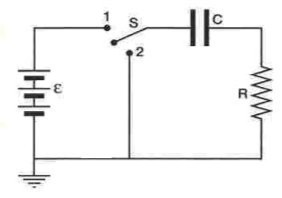
\includegraphics[width=0.30\textwidth]{imágenes/capacitor/circuito.jpg}
			\caption{Circuito a montar para estudiar el comportamiento de un capacitor al cargar y descargarlo.}
			\label{fig:circuito_capacitor}
		\end{figure}

		Se utilizaron valores de resistencia y capacitor de 1$k\Omega$, 581 $\mu F$ con constante de tiempo $\tau =$ 581 $ms$ y
		10 $k\Omega$, 980 $\mu F$ con constante de tiempo $\tau =$ 9.8 $s$, respectivamente para el primer y segundo montaje.\\

		Al conectar una fuente a 1 $V$ para cada uno de los montajes, se observó el comportamiento mostrado en la Figura \ref{fig:CyD},
		donde se logra apreciar las curvas tanto de carga como de descarga de los capacitores asi como los cursores del osciloscopio
		que muestran la diferencia temporal, donde el primer cursor esta colocado en el inicio de la carga o descarga y el segundo
		cursor colocado cuando la carga llega al 63.2 \% de la carga total esperada al cargar, es decir, 1 $V$, y cuando la carga
		llega al 36.8 \% de su carga total al descargar.\\

		Por casi todos los resultados obtenidos en la Figura \ref{fig:CyD} y los valores esperados calculados, los resultados fueron
		como lo esperado así como el comportamiento del voltaje para la carga y descarga de un capacitor.\\
		Como observación, al disminuir o aumentar el voltaje proporcionado por la fuente, teniendo cuidado del voltaje nominal del capacitor,
		solo cambió la amplitud del voltaje que recibe el capacitor, es decir, que el capacitor iguala el voltaje que se le proporciona.\\

		\begin{figure}[!ht]
			\centering

			% Primera fila
			\begin{subfigure}[b]{\linewidth}
				\centering
				
				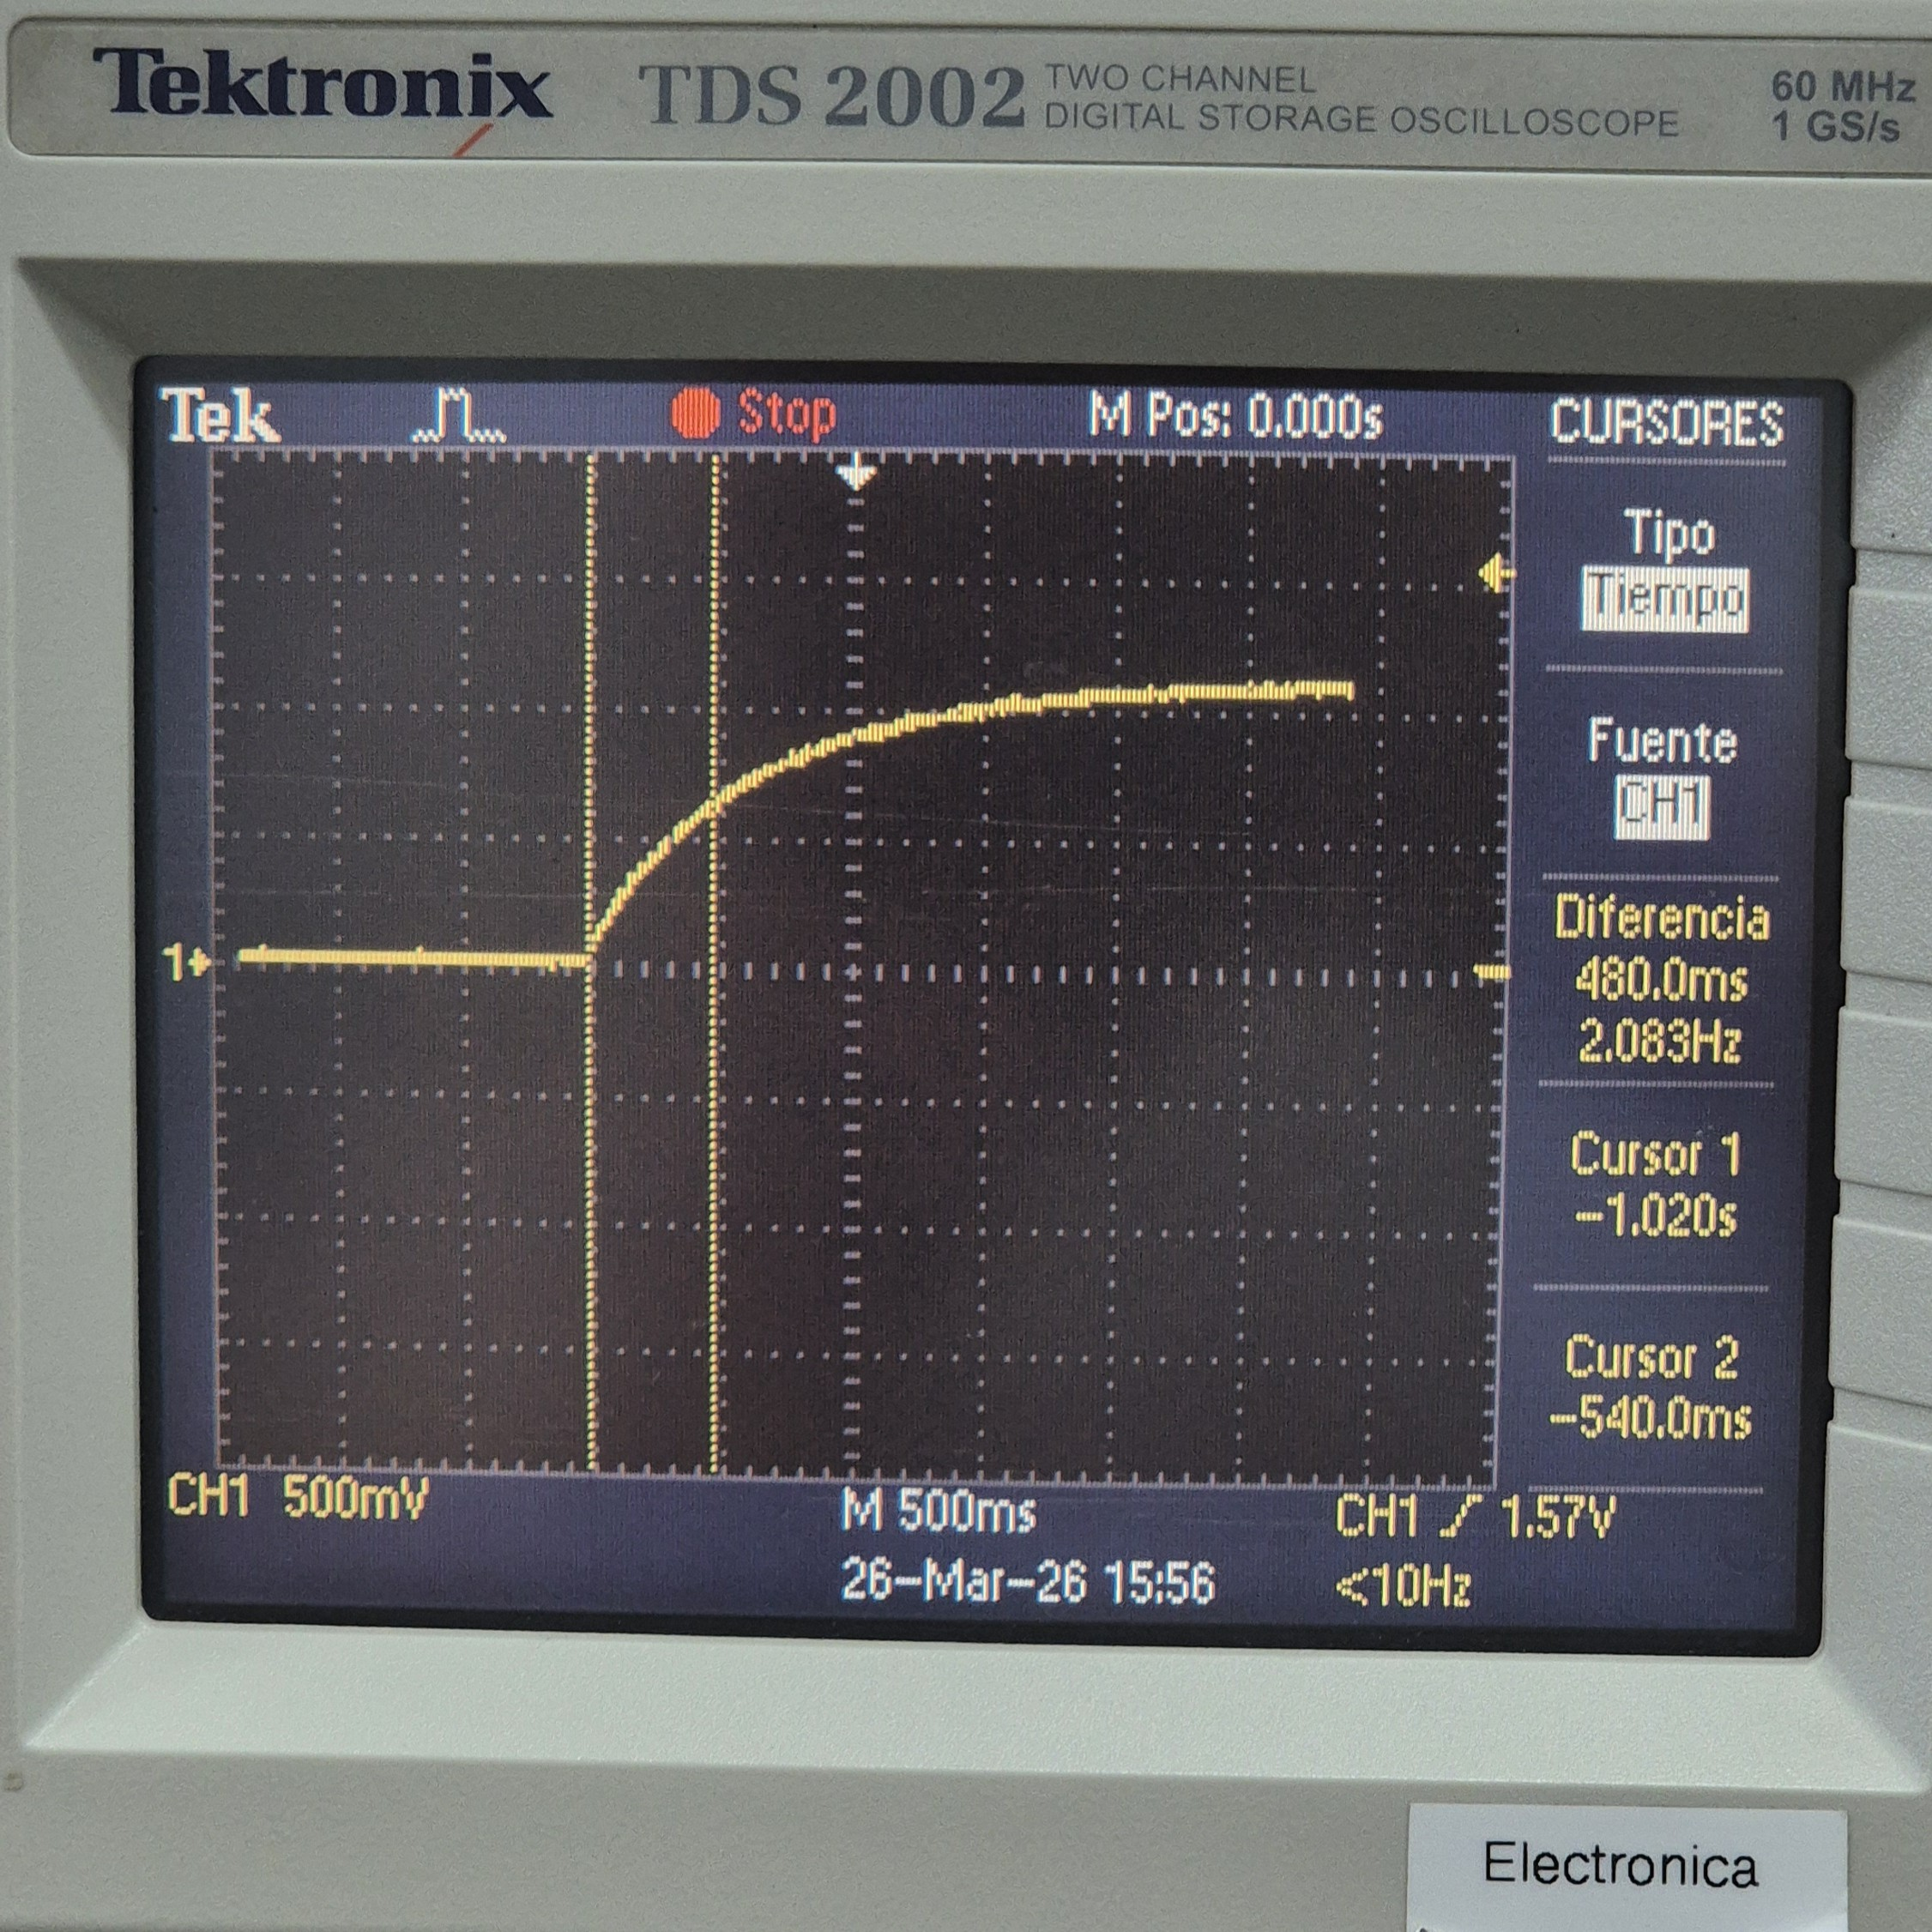
\includegraphics[width=0.49\linewidth]{imágenes/capacitor/carga1.jpg}
				\hfill
				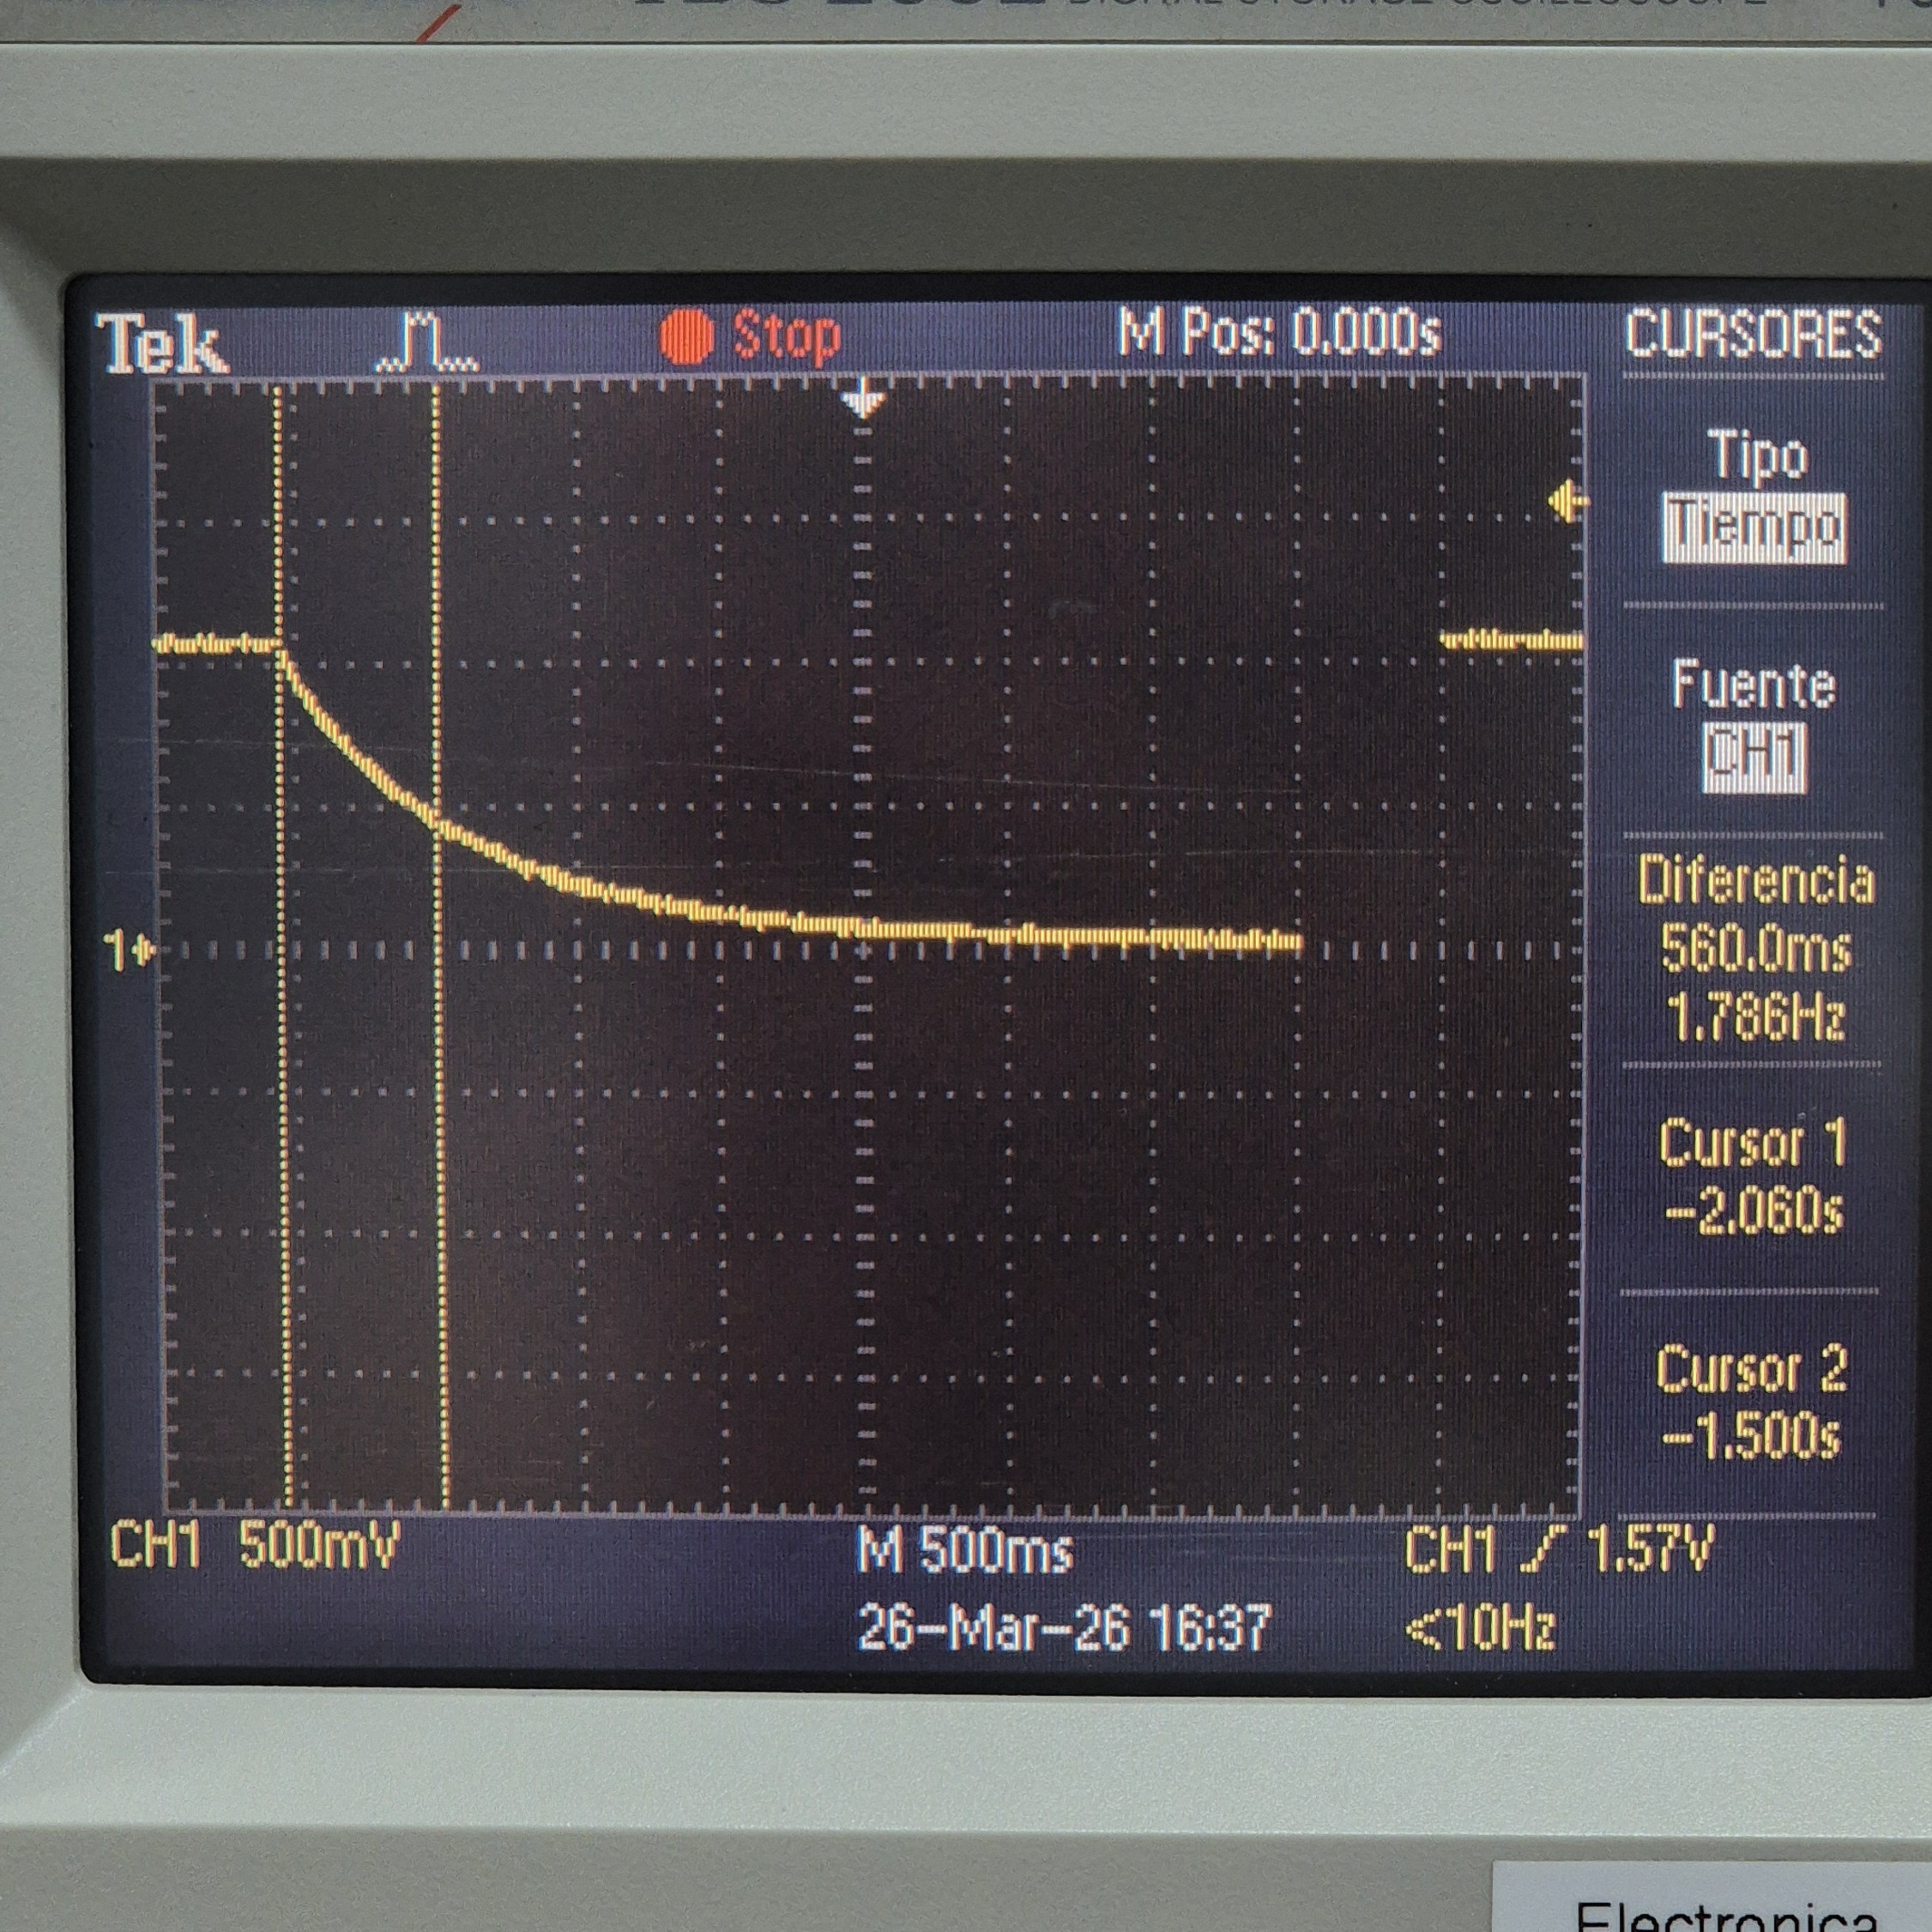
\includegraphics[width=0.49\linewidth]{imágenes/capacitor/descarga1.jpg}

				\caption{Primer montaje con constante de tiempo de 581 $ms$.}
			\end{subfigure}

			\vspace{0.5mm}

			% Segunda fila
			\begin{subfigure}[b]{\linewidth}
				\centering
				
				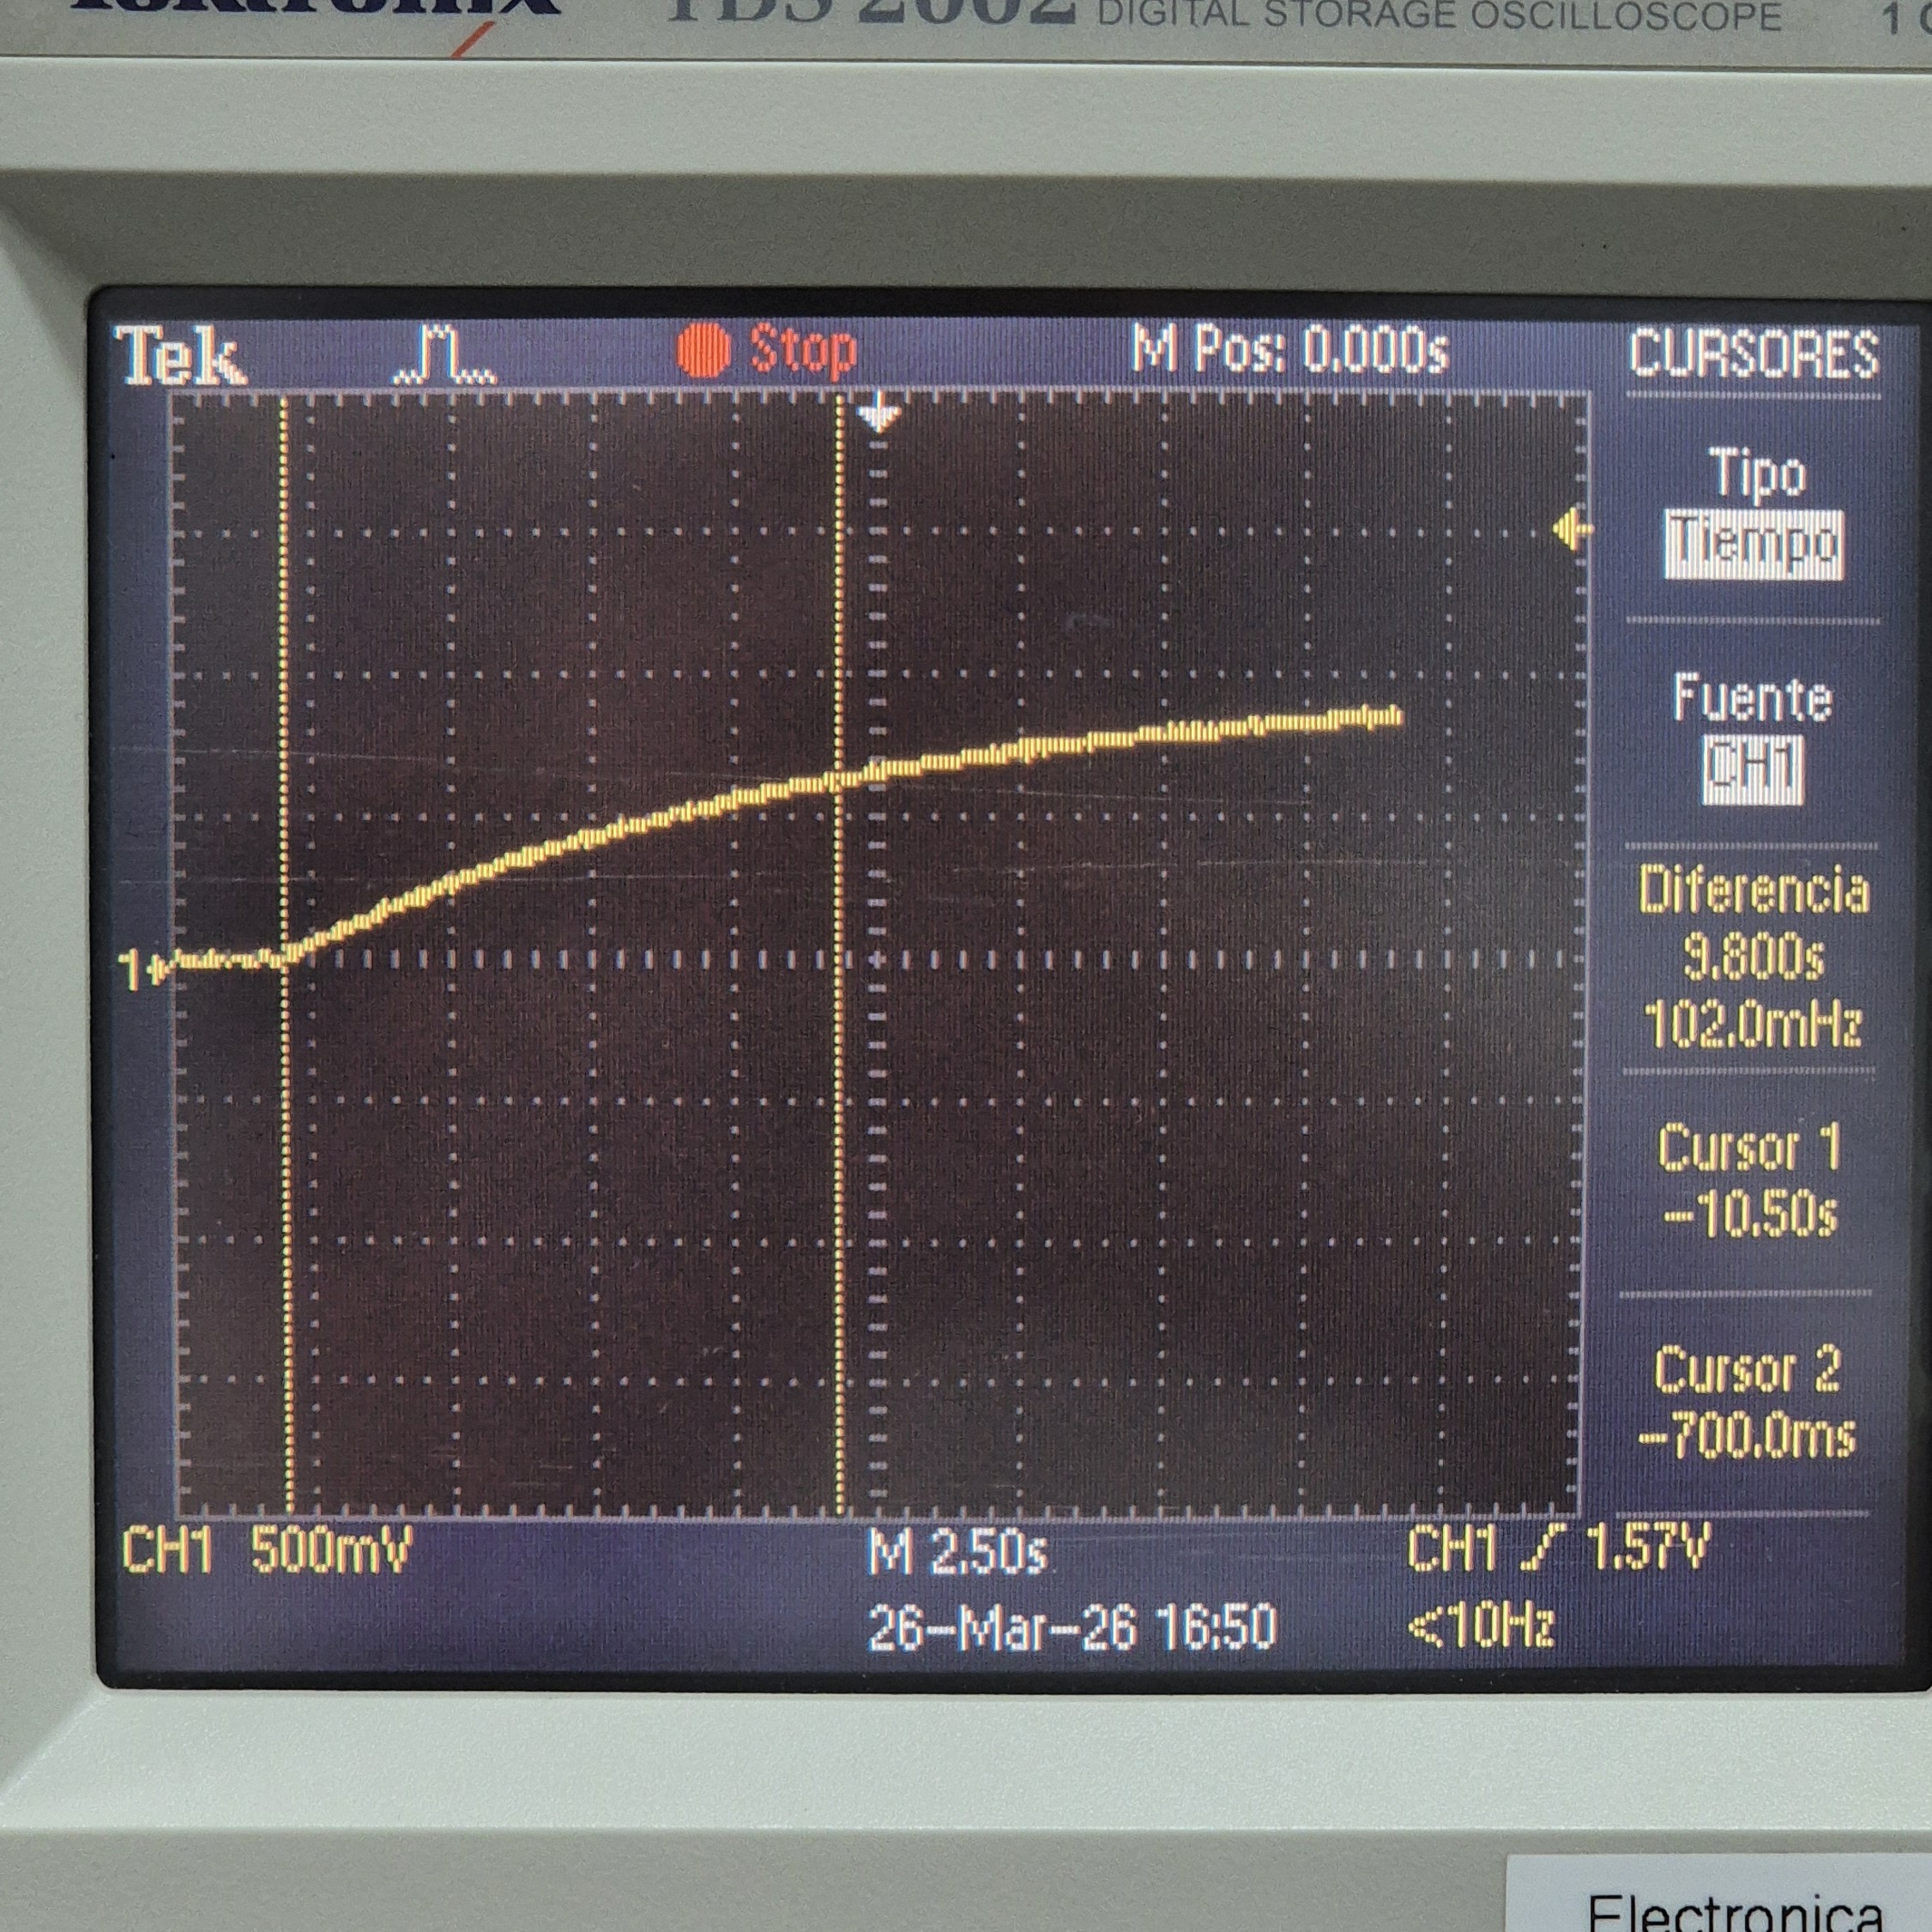
\includegraphics[width=0.49\linewidth]{imágenes/capacitor/carga2.jpg}
				\hfill
				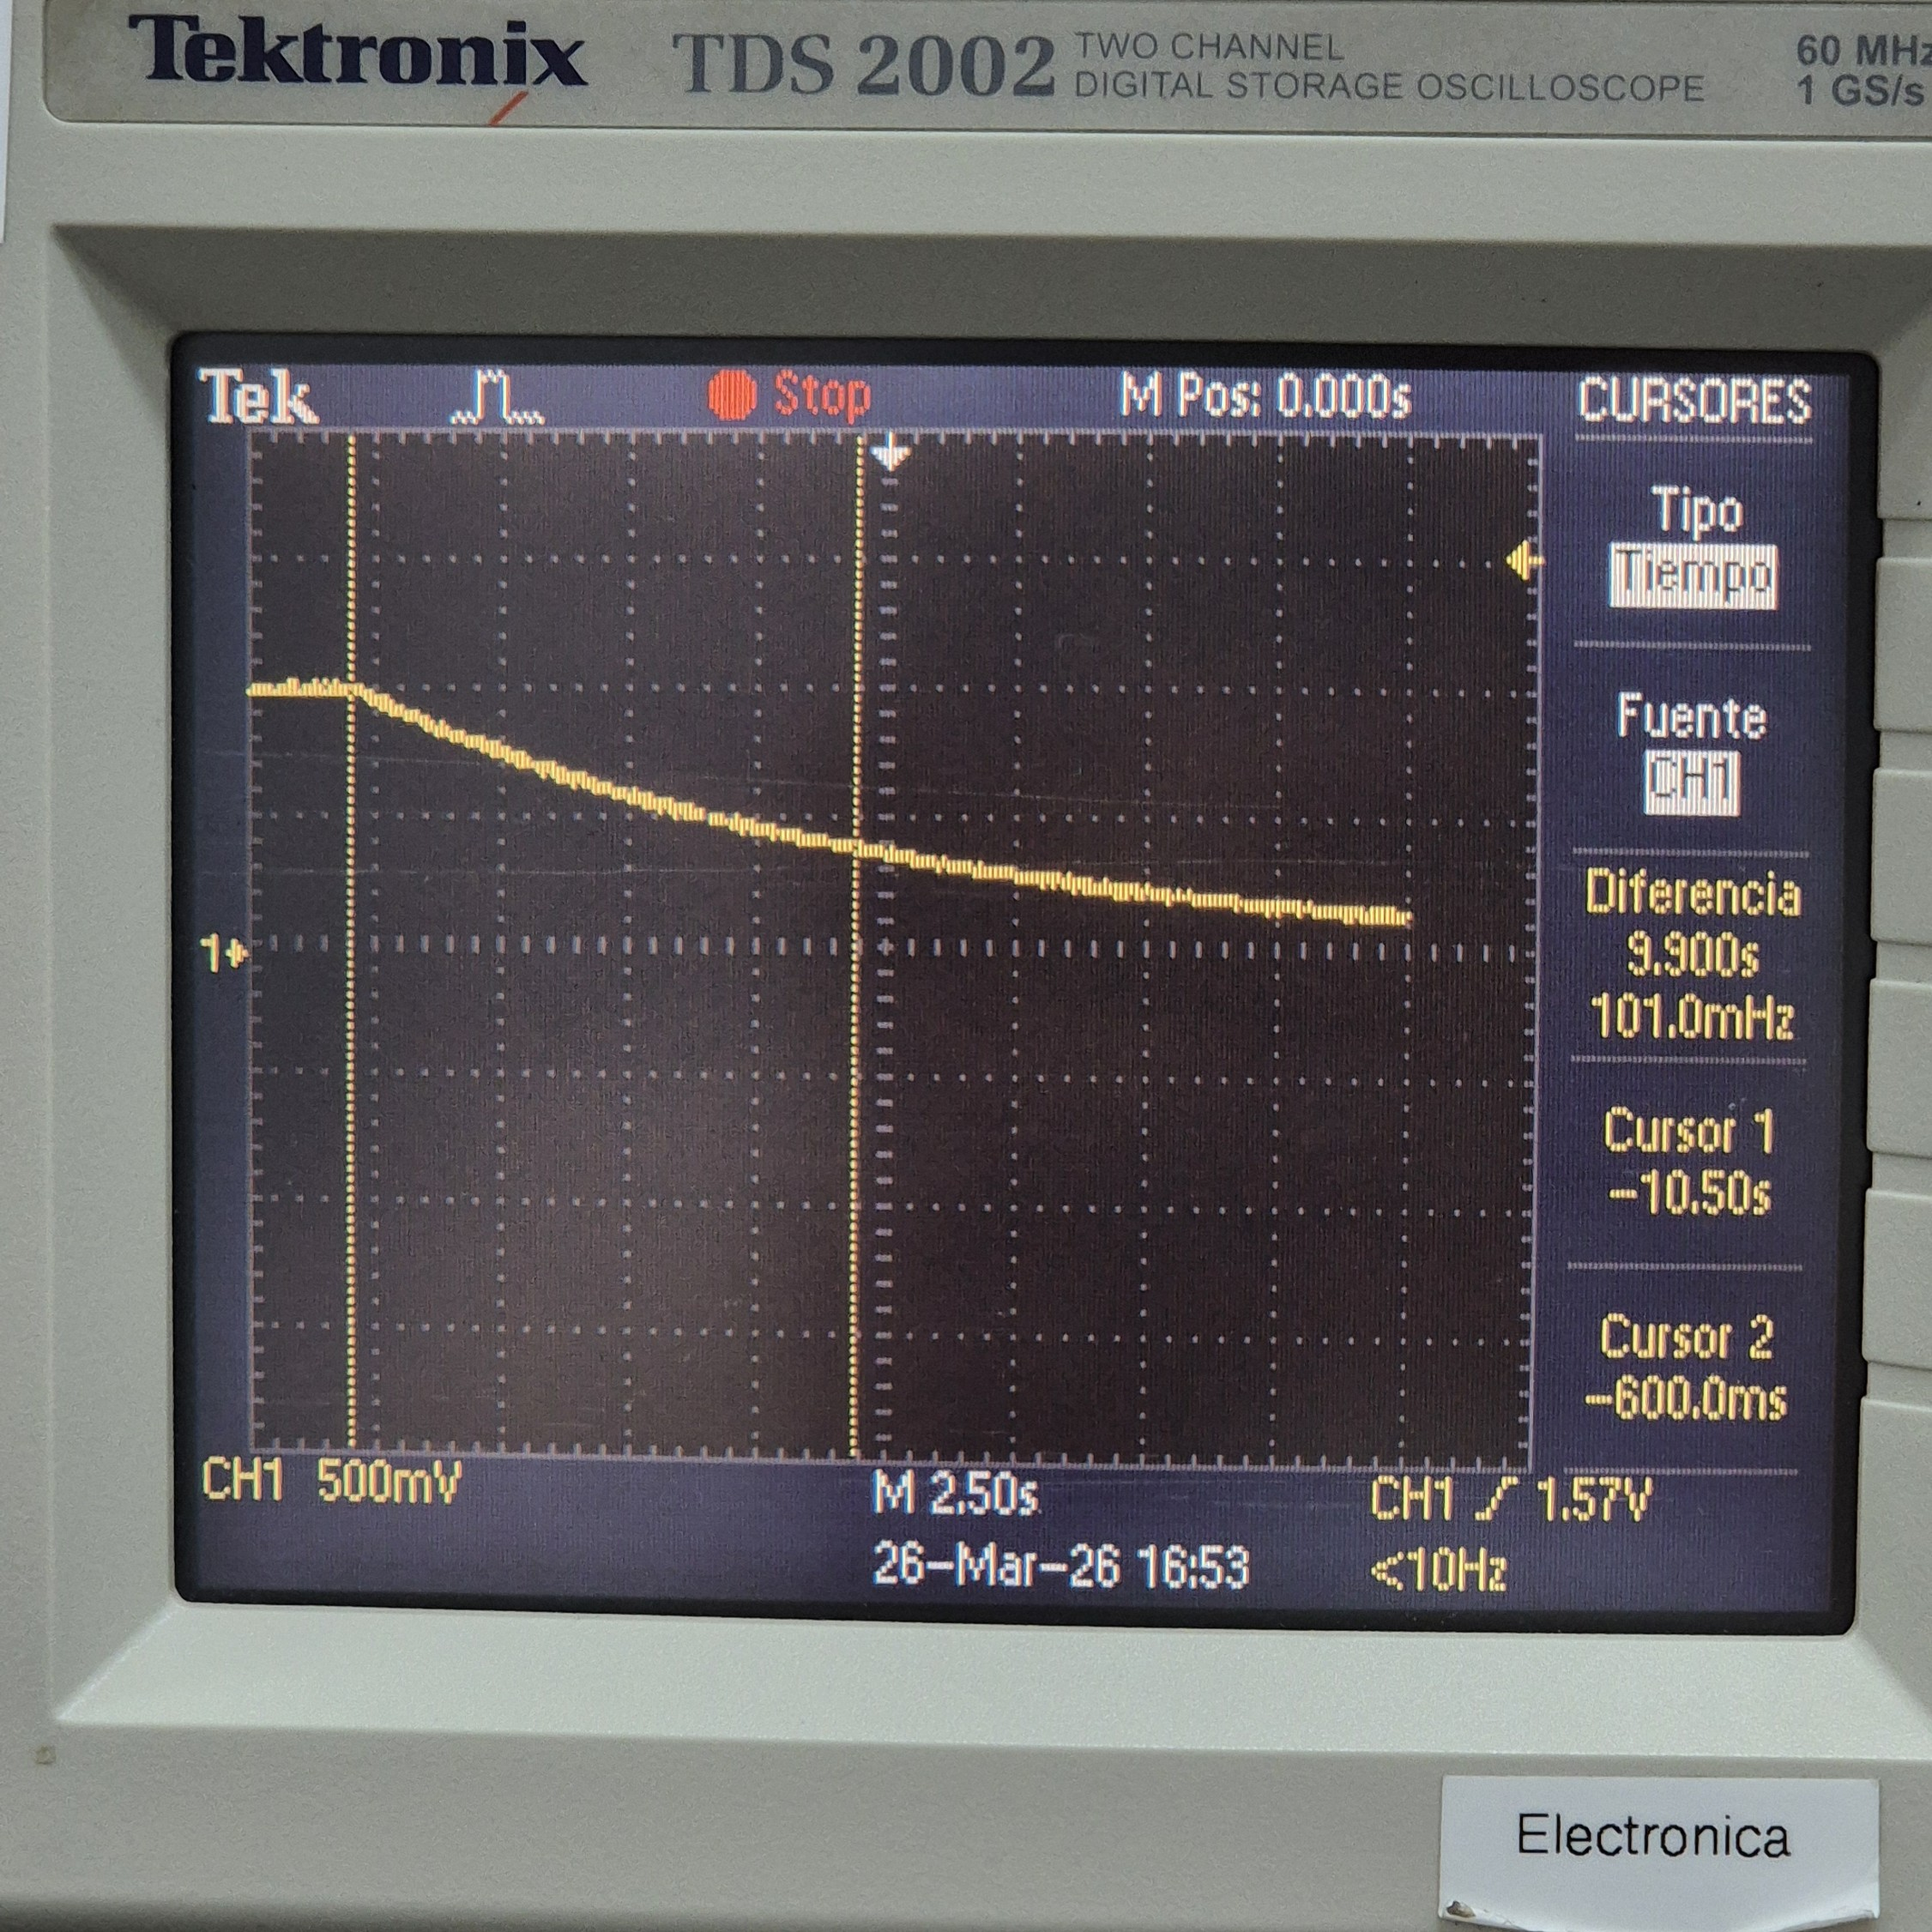
\includegraphics[width=0.49\linewidth]{imágenes/capacitor/descarga2.jpg}

				\caption{Segundo montaje con constante de tiempo de 9.8 $s$.}
			\end{subfigure}

			\caption{Montaje de dos circuitos para la carga y descarga de un capacitor con distintas constantes de tiempo.}
			\label{fig:CyD}

		\end{figure}
		
		Es importante destacar que la primer imagen de la Figura \ref{fig:CyD} se puede ver que el valor de $\tau$ no coincide con
		el valor esperado pues no se usó el switch mostrado en la Figura \ref{fig:circuito_capacitor}, y por ello dio otro valor
		al esperado, es por eso que para los siguientes montajes ya se consideró este switch que se muestra en la Figura \ref{fig:CyD}
		dando mucho mejores resultados.

	\section{Fuente DC lineal}
		Para esta sección, el objetivo fue realizar una fuente lineal DC montando el circuito de la Figura \ref{fig:circuito_DC}
		dividido en cuatro etapas, las cuales son:

		\begin{figure}[!ht]
				\centering
				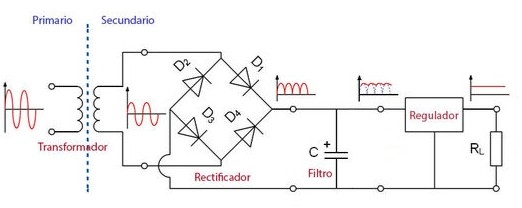
\includegraphics[width=0.48\textwidth]{imágenes/fuente DC/circuito_fuenteDC.jpg}
				\caption{Circuito a montar para elaborar una Fuente DC lineal.}
				\label{fig:circuito_DC}
			\end{figure}

		\subsection{Transformación}
			La primera etapa consiste en usar un Transformador pues el objetivo es llevar a la señal de la linea, la cual esta a
			aproximadamente 127 $V$ 60 $Hz$, a una señal DC, por lo que el transformador sirve como un atenuador de amplitud de la señal,
			pues deja la frecuencia intacta y lleva el voltaje de la señal a su voltaje nominal.\\

			En nuestro caso usamos un Transformador con tap central de 12 $V$ 1$A$ que, usando únicamente las entradas de los extremos,
			nos llevo realmente a un valor de 14 $V_RMS = $ 20 $V_{PP}$ como se logra apreciar en la Figura \ref{fig:transformador}.

			\begin{figure}[!ht]
				\centering
				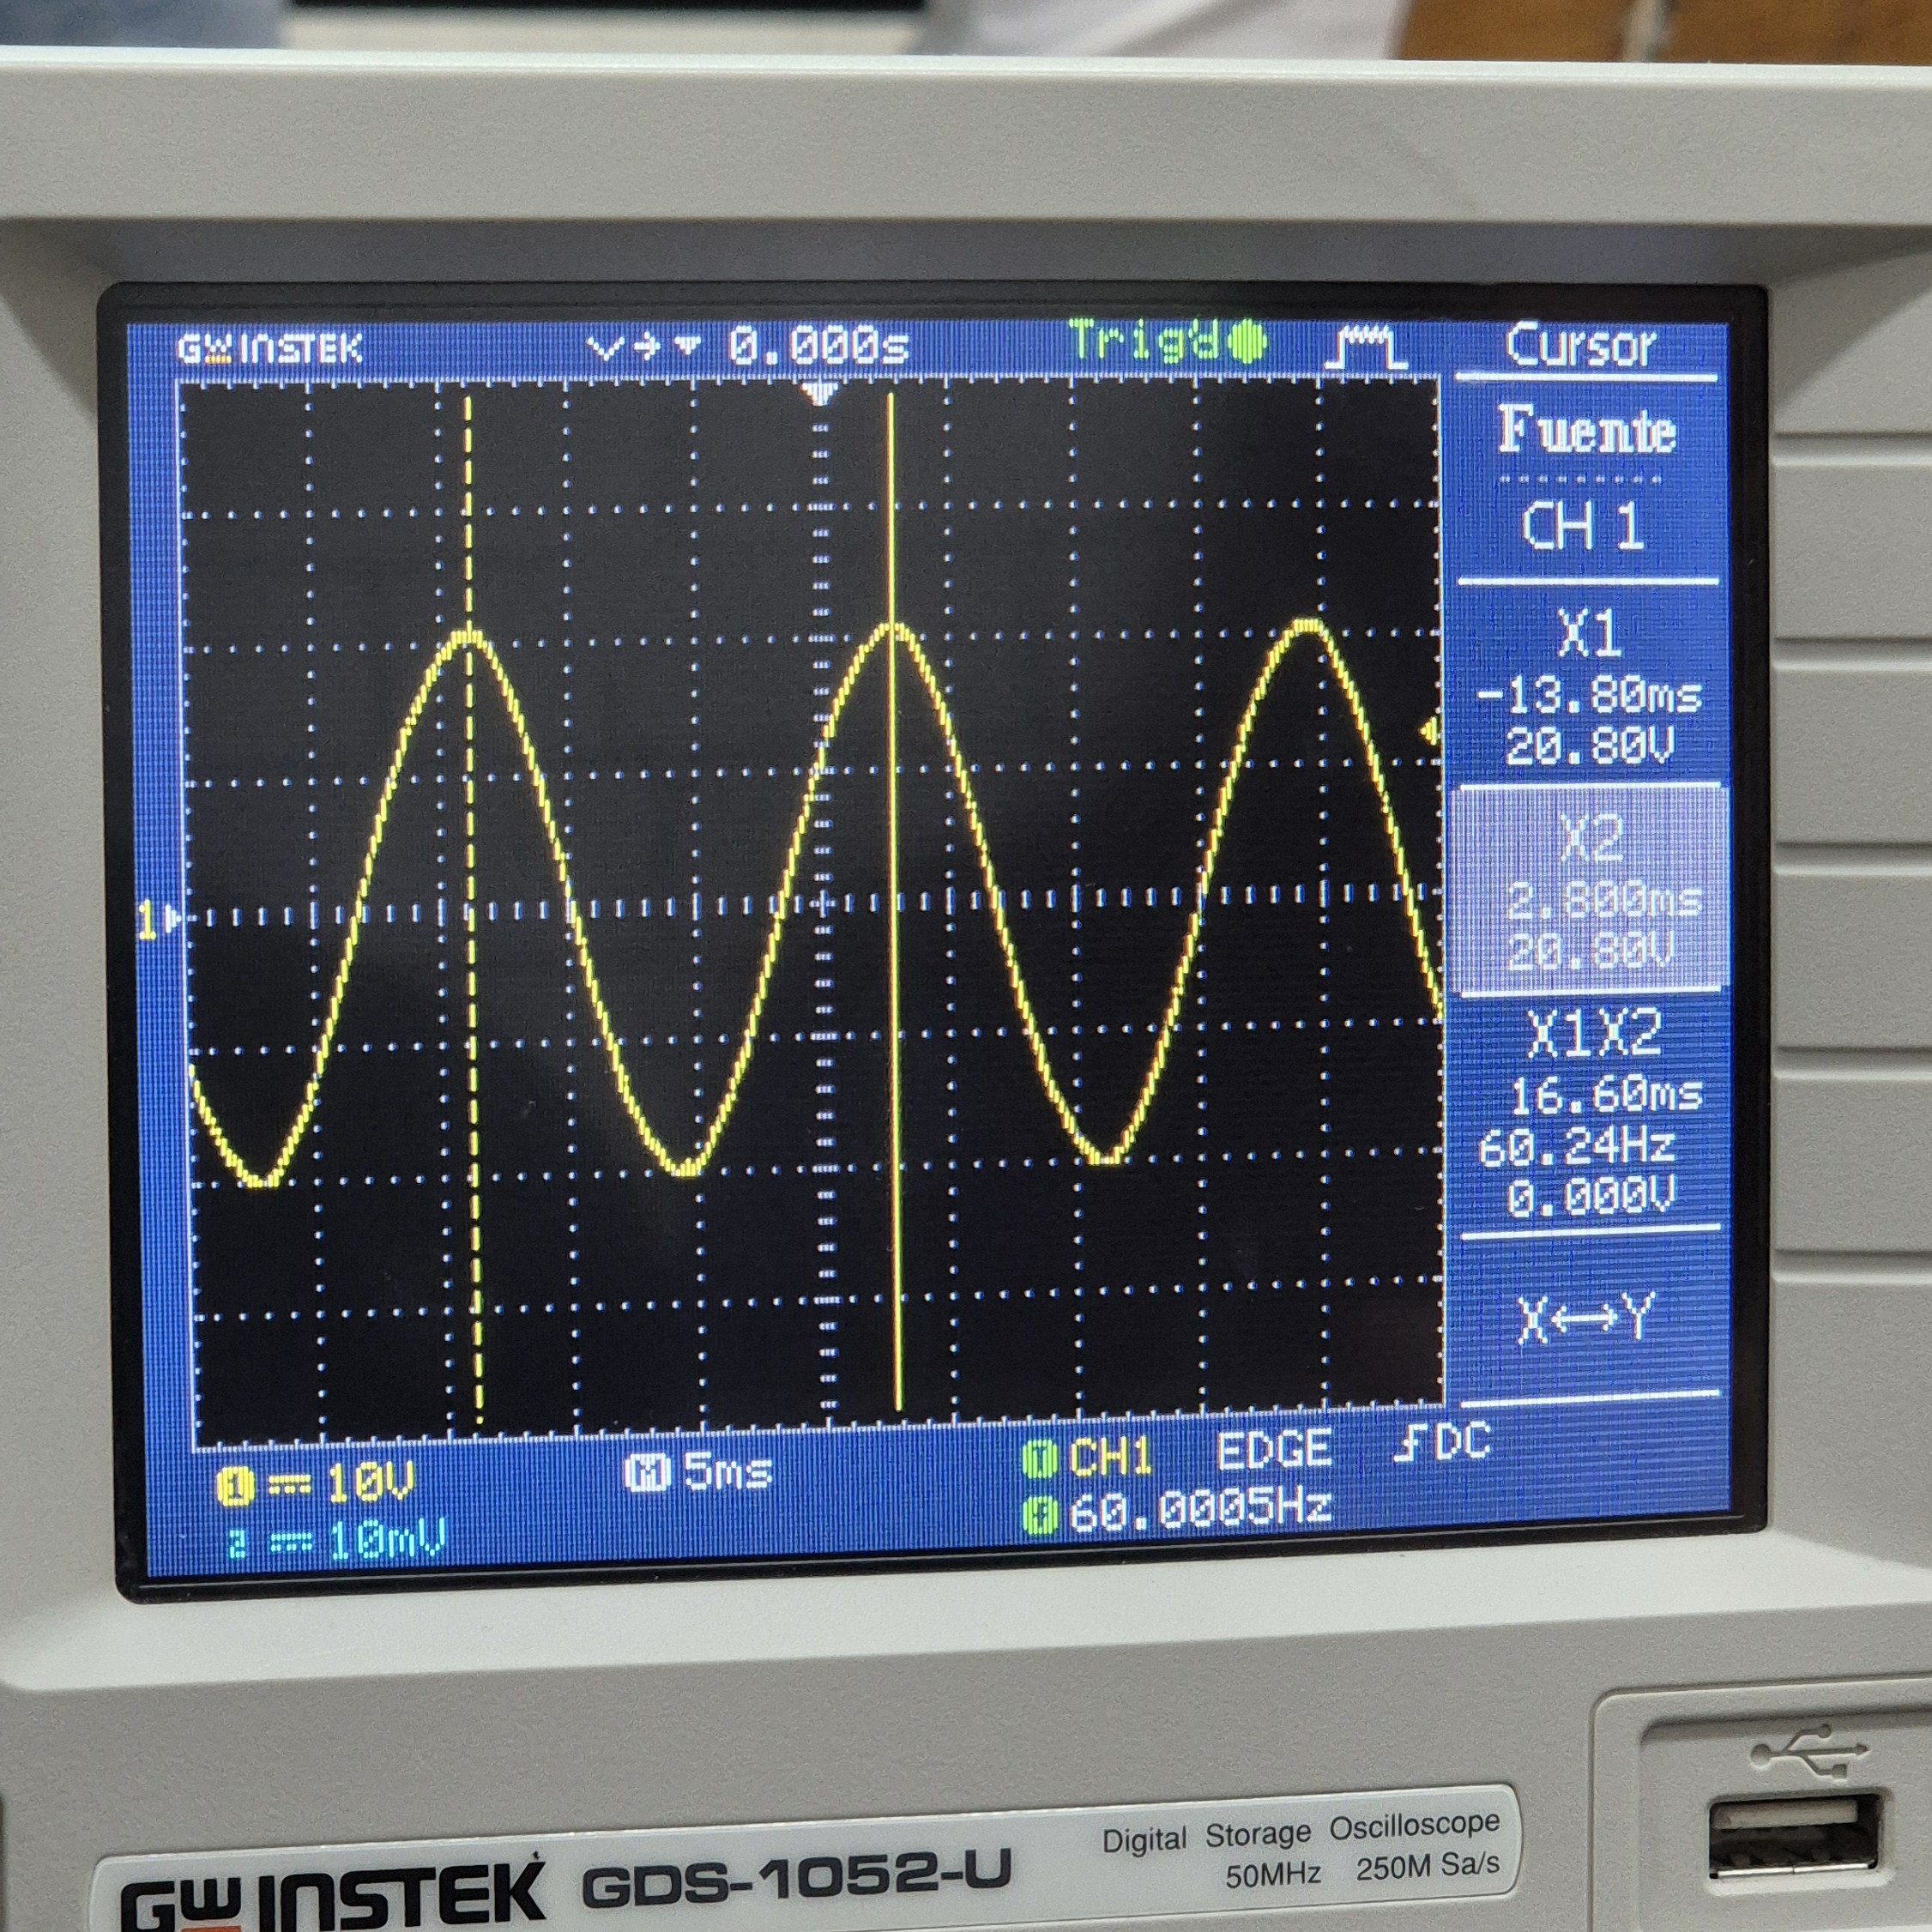
\includegraphics[width=0.42\textwidth]{imágenes/fuente DC/transformación.jpg}
				\caption{Señal obtenida luego de la transformación de la señal de la linea con un Transofrmador de 12 $V$.}
				\label{fig:transformador}
			\end{figure}

		\subsection{Rectificación}
			Los diodos son semiconductores que funcionan como un interruptor unidireccional permitiendo que la corriente fluya solo
			en una dirección, más especificamente del ánodo al cátodo, y bloqueándola en la dirección contraria. Para esta etapa el
			objetivo principal fue armar un puente rectificador de diodos de onda completa, para lo cual se usaron 4 diodos 1N4004
			acomodados como se muestra en la Figura \ref{fig:puente_diodos} de tal manera que la señal AC atenuada por el Transformador
			se convirtió en una señal de voltaje DC \textbf{pulsante} como se muestra en la Figura \ref{fig:onda_completa}.

			\begin{figure}[!ht]
				\centering
				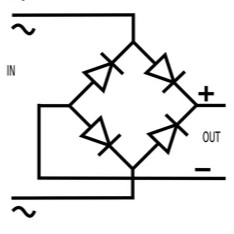
\includegraphics[width=0.25\textwidth]{imágenes/fuente DC/puente.jpg}
				\caption{Puente rectificador de diodos de onda completa.}
				\label{fig:puente_diodos}
			\end{figure}

			\begin{figure}[!ht]
				\centering
				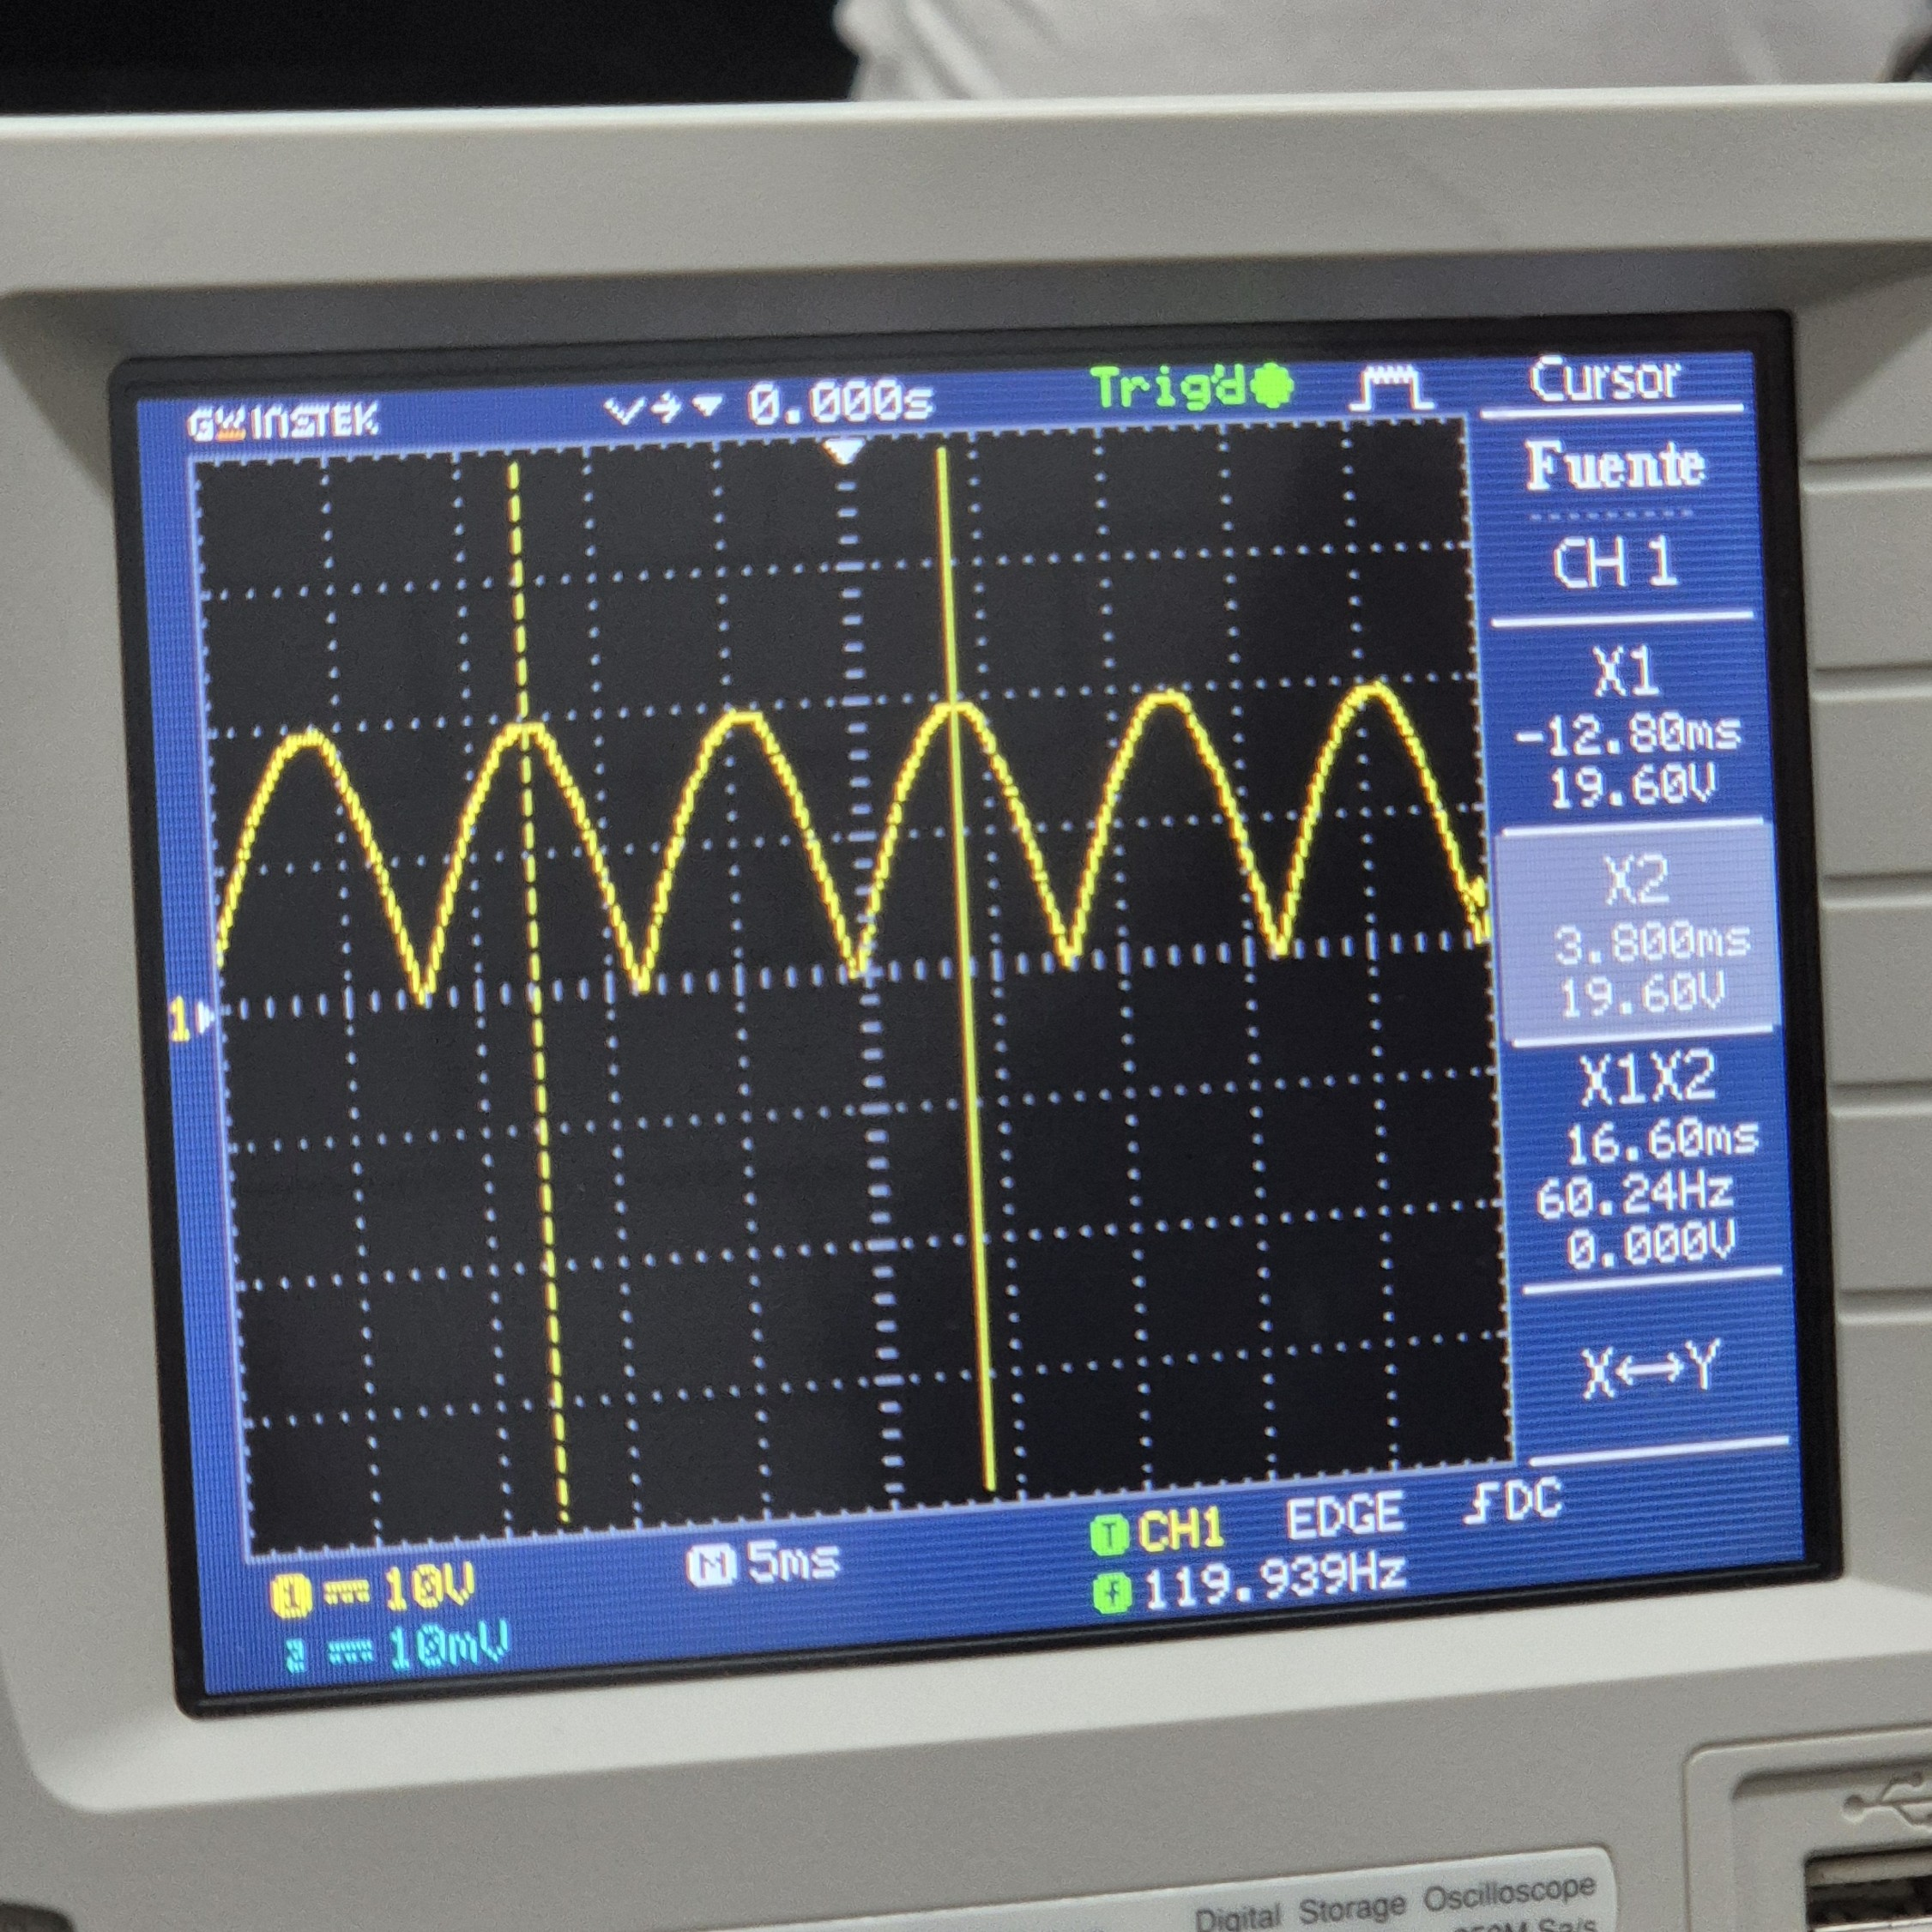
\includegraphics[width=0.42\textwidth]{imágenes/fuente DC/rectificación.jpg}
				\caption{Señal obtenida luego de la rectificación por un puente de 4 diodos.}
				\label{fig:onda_completa}
			\end{figure}

		\subsection{Filtraje}
			Posterior a la rectificación le sigue el uso de un filtro, en nuestro caso usamos un capacitor de 4700 $\mu F$, junto con
			una resistencia de 3.9 $k\Omega$, pues fue el que dio mejores resultados a diferencia de otros de valor 1 y 220 $\mu F$
			los cuales dieron la Figura \ref{fig:filtraje1} como resultado.

			\begin{figure}[!ht]
				\centering
				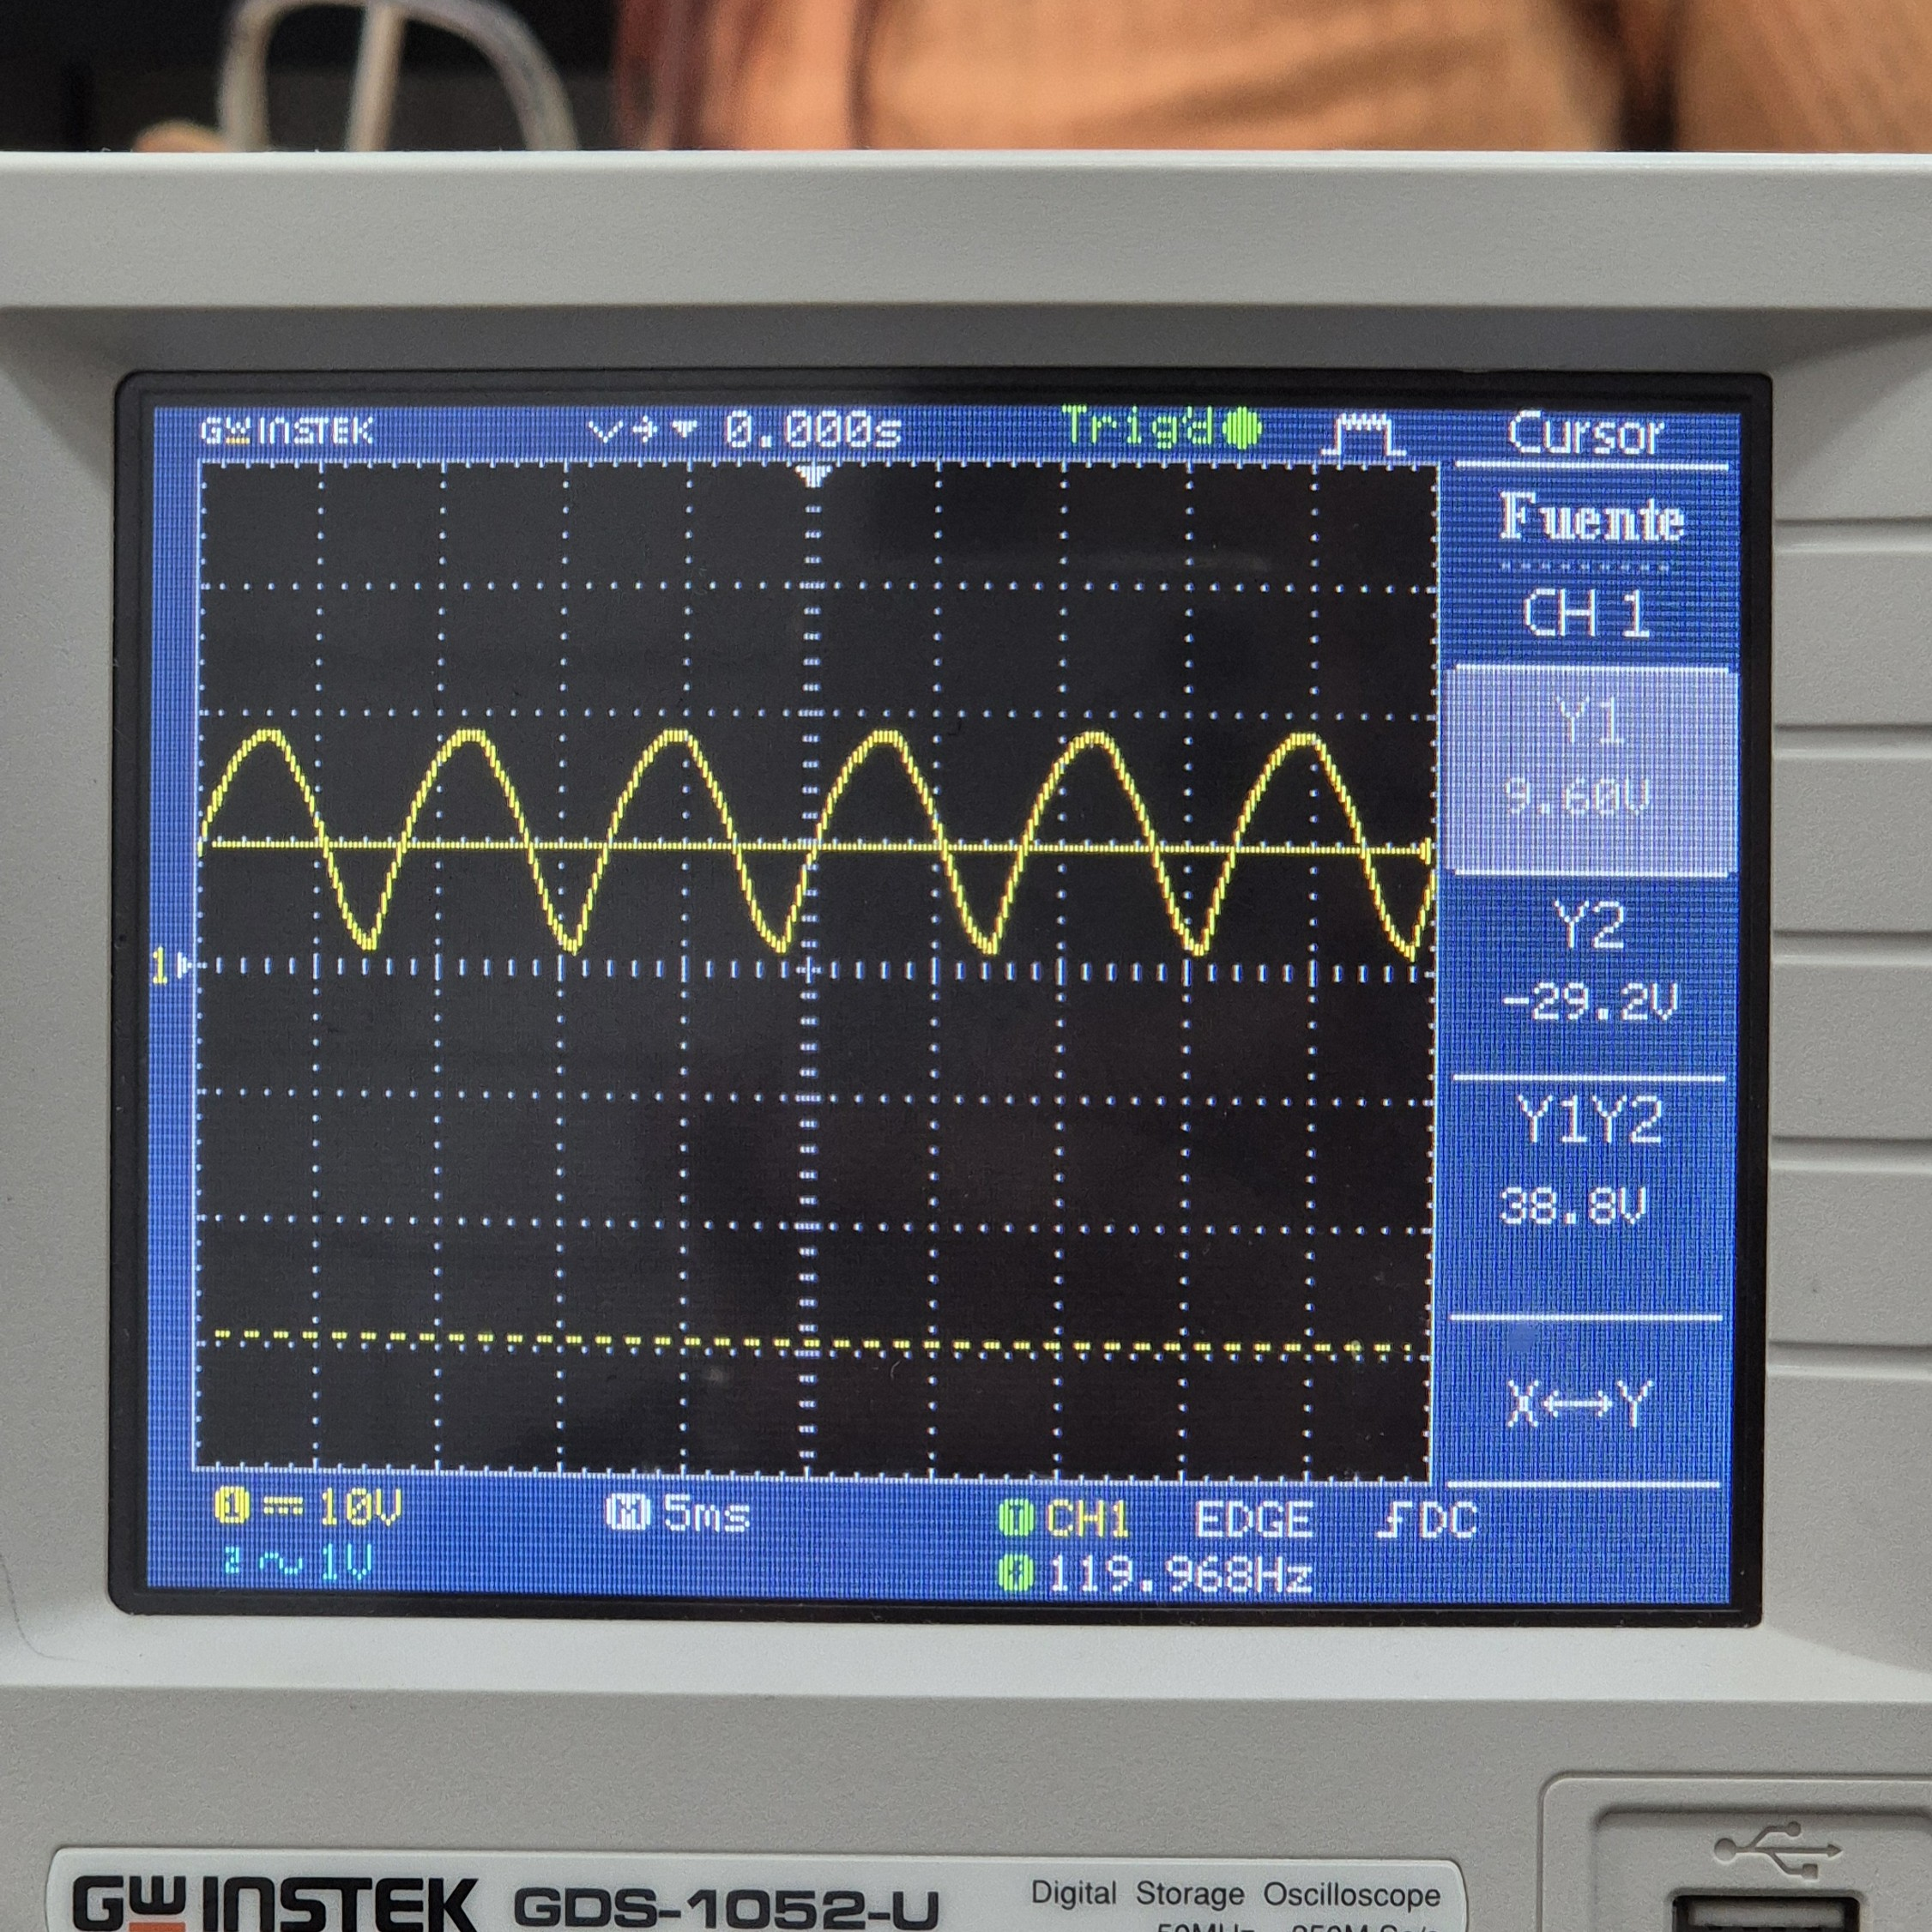
\includegraphics[width=0.48\linewidth]{imágenes/fuente DC/filtraje1.jpg}
				\hfill
				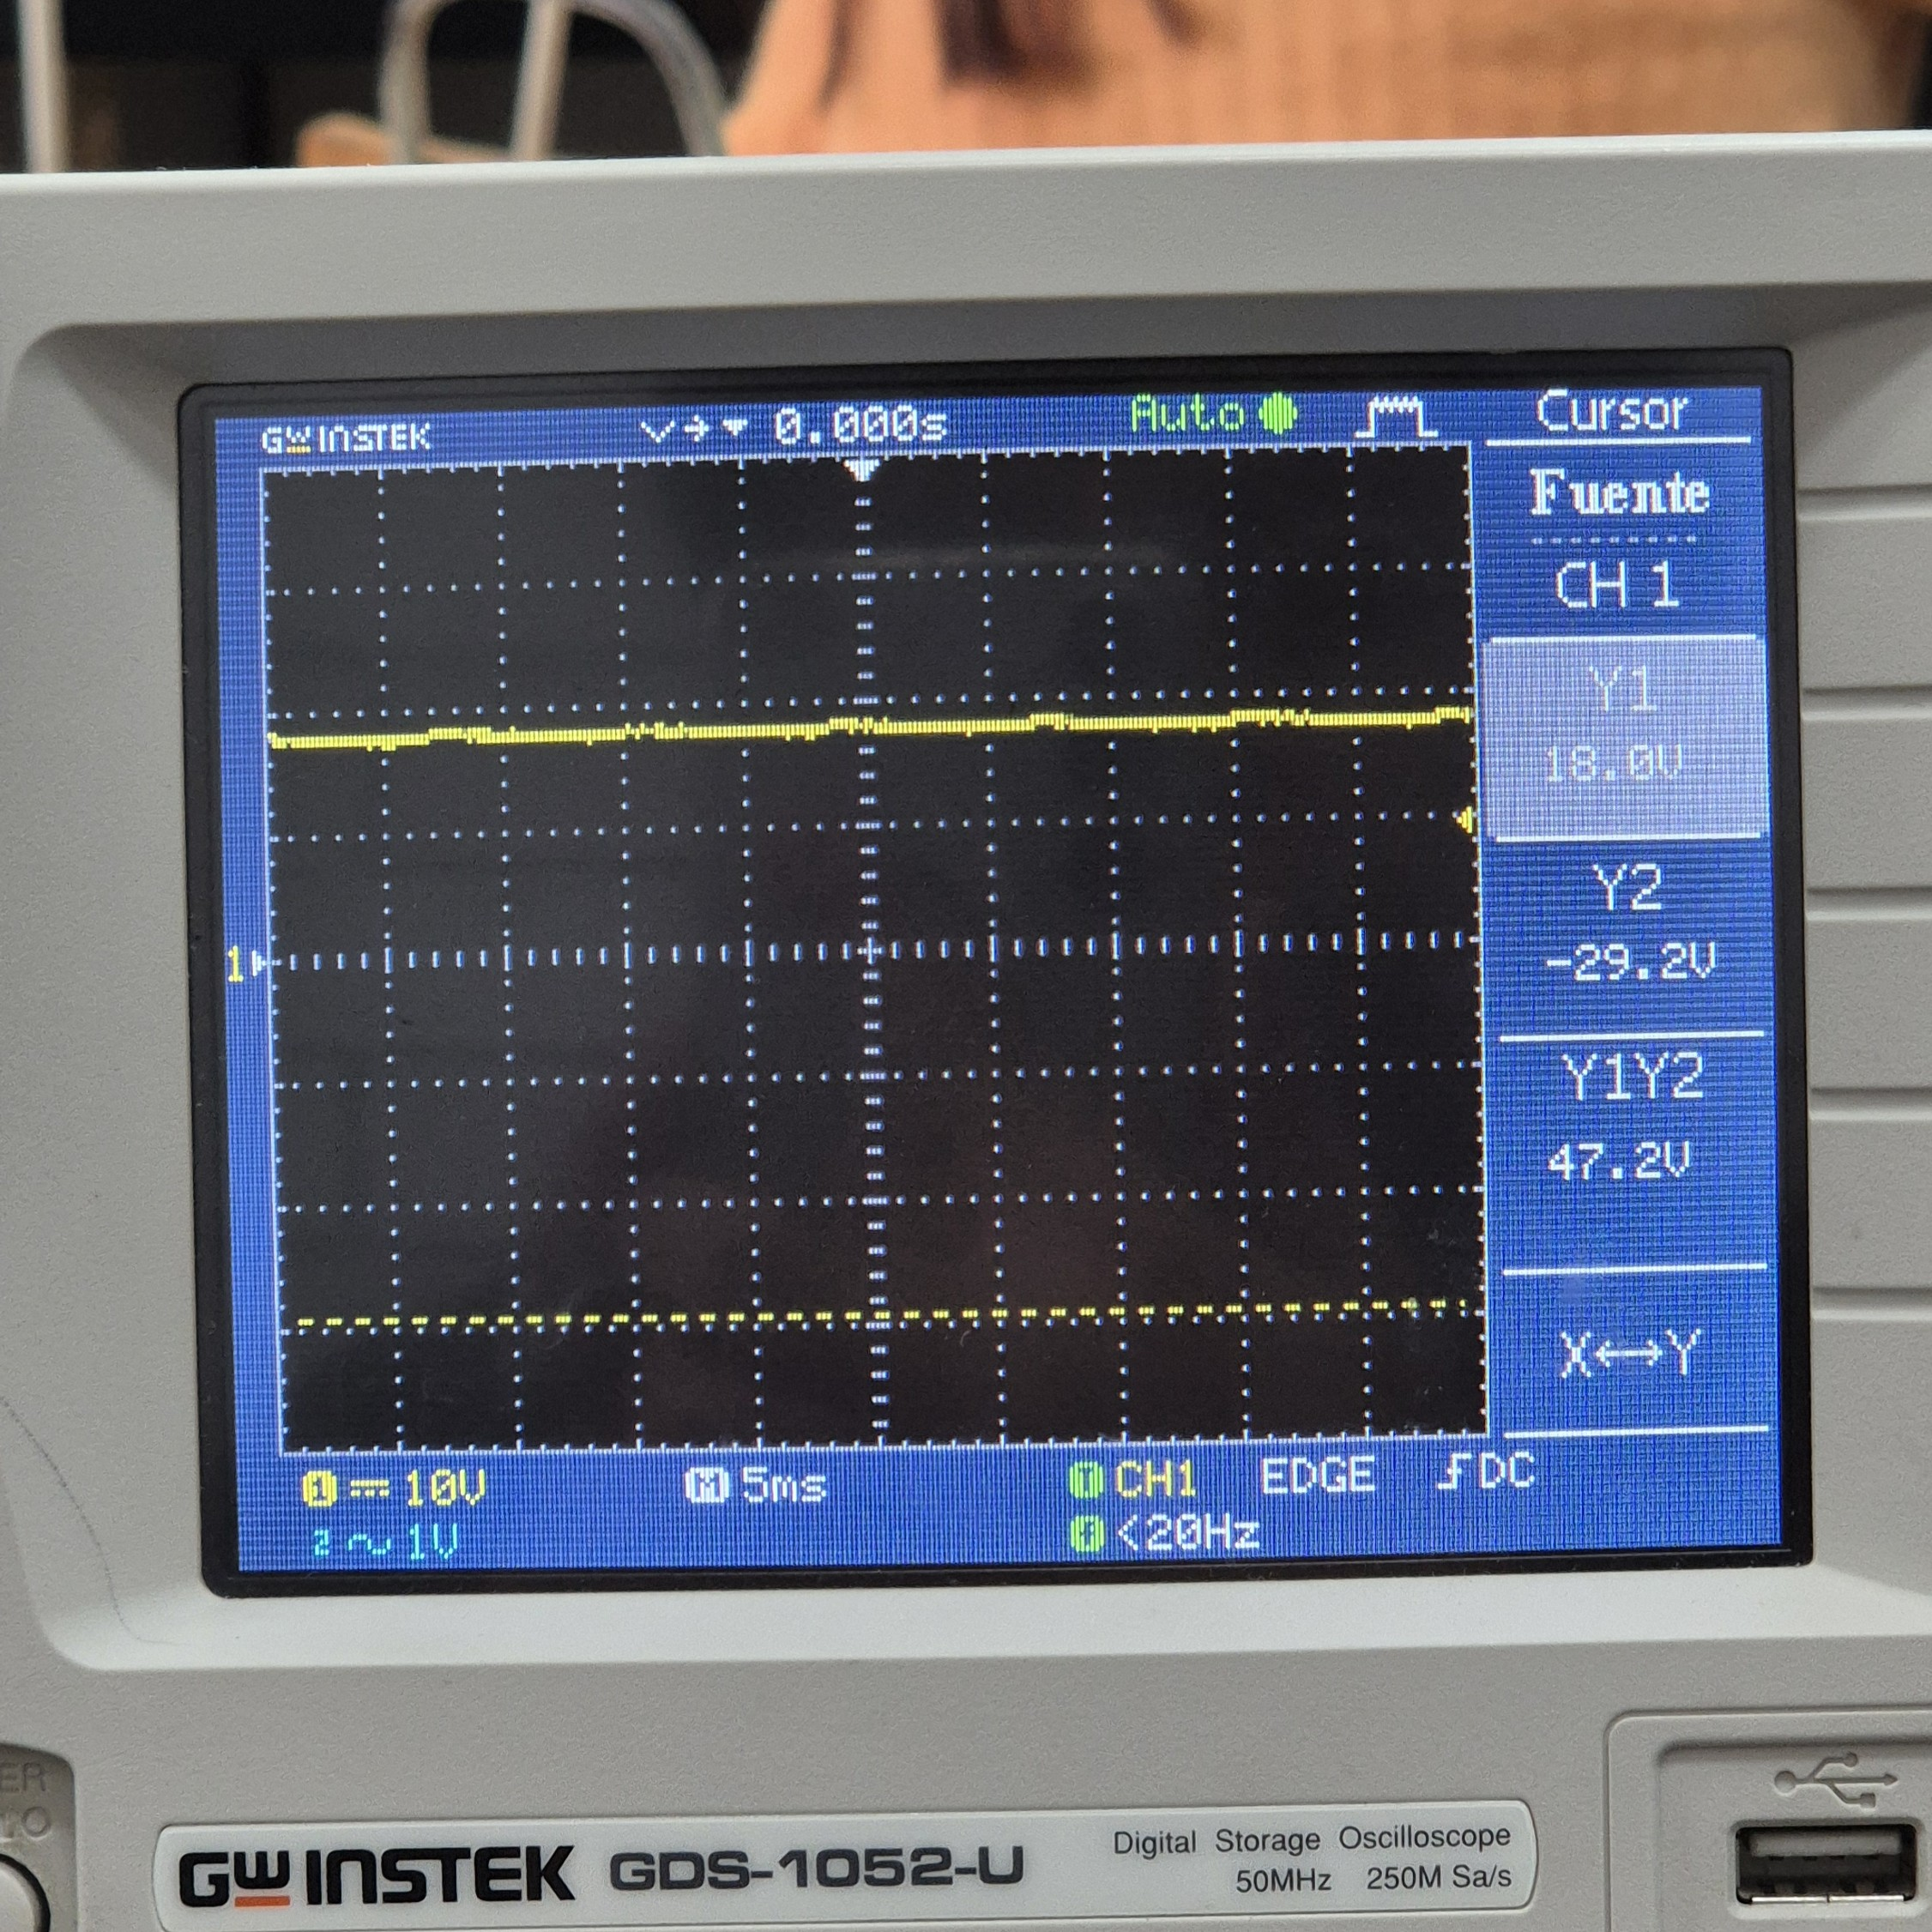
\includegraphics[width=0.48\linewidth]{imágenes/fuente DC/filtraje2.jpg}

				\caption{Señales de prueba obtenidas en el filtraje con capacitores de 1 y 220 $\mu F$, respectivamente.}
				\label{fig:filtraje1}
			\end{figure}

			El capacitor funciona como un filtro que, dado que este componente usa su energía almacenada de acuerdo a como el circuito
			lo demande, cuando la señal DC pulsante tiene una pendiente positiva el capacitor se carga y cuando la pendiente es negativa
			este se descarga de tal manera que elimina gran parte de los ``rizos'' de la señal como lo obtenido en la Figura \ref{fig:filtraje3}.

			\begin{figure}[!ht]
				\centering
				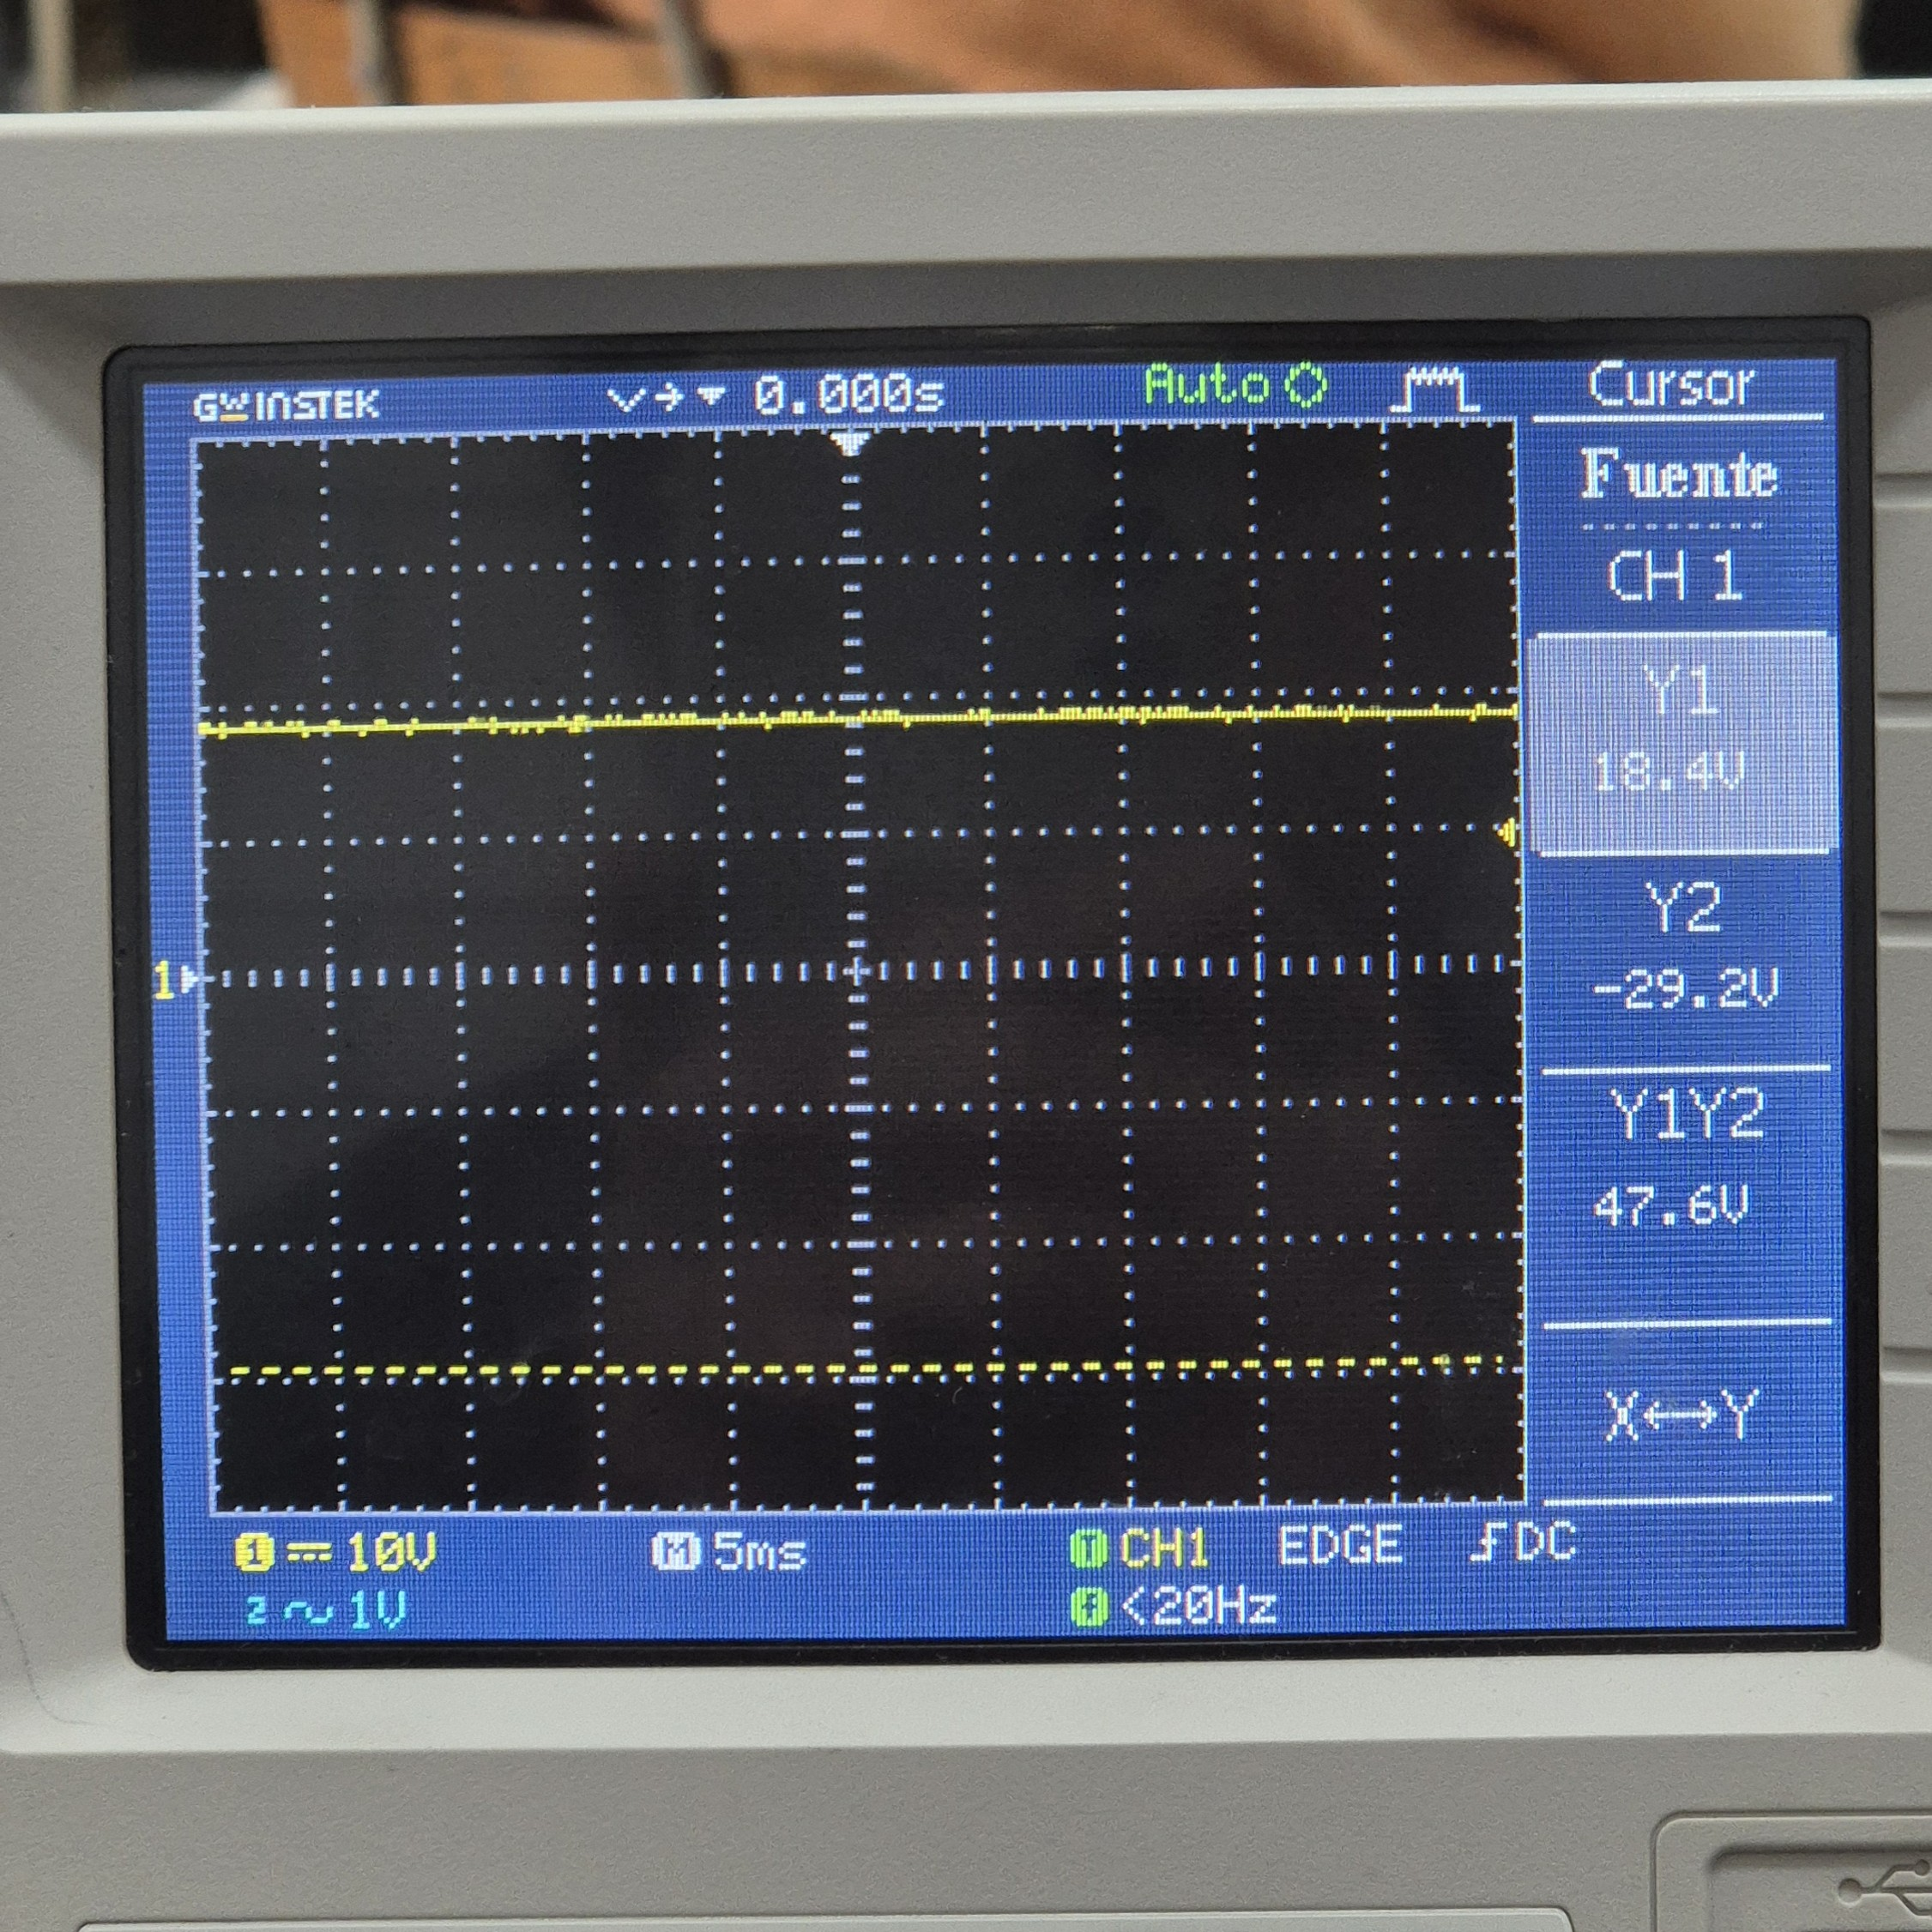
\includegraphics[width=0.42\textwidth]{imágenes/fuente DC/filtraje3.jpg}
				\caption{Señal obtenida luego del Filtraje con un capacitor de 4700 $\mu F$.}
				\label{fig:filtraje3}
			\end{figure}

		\subsection{Regulación}
			Por último, para eliminar los rizos restantes que pudieron haber quedado de la etapa anterior se usó un regulador 7812,
			que en general, tiene como regla que el voltaje que le entra a este debe ser mayor al voltaje de salida, de cualquier manera
			es recomendable revisar datasheets para corroborar los valores que puede recibir el regulador así como lo que representa
			cada terminal de este.\\
			Para un mejor rendimiento del regulador, se conectaron dos capacitores de valores 100 $nF$ y 1 $\mu F$ a este, de manera que
			el de mayor valor este conectado al input y el de menor valor al output.\\

			Por lo cual, finalmente, con todas las etapas convertimos la señal de la linea a una señal DC estable de 12.2 $V$ como
			se muestra en la Figura \ref{fig:regulador} y como se tenía de objetivo.

			\begin{figure}[!ht]
				\centering
				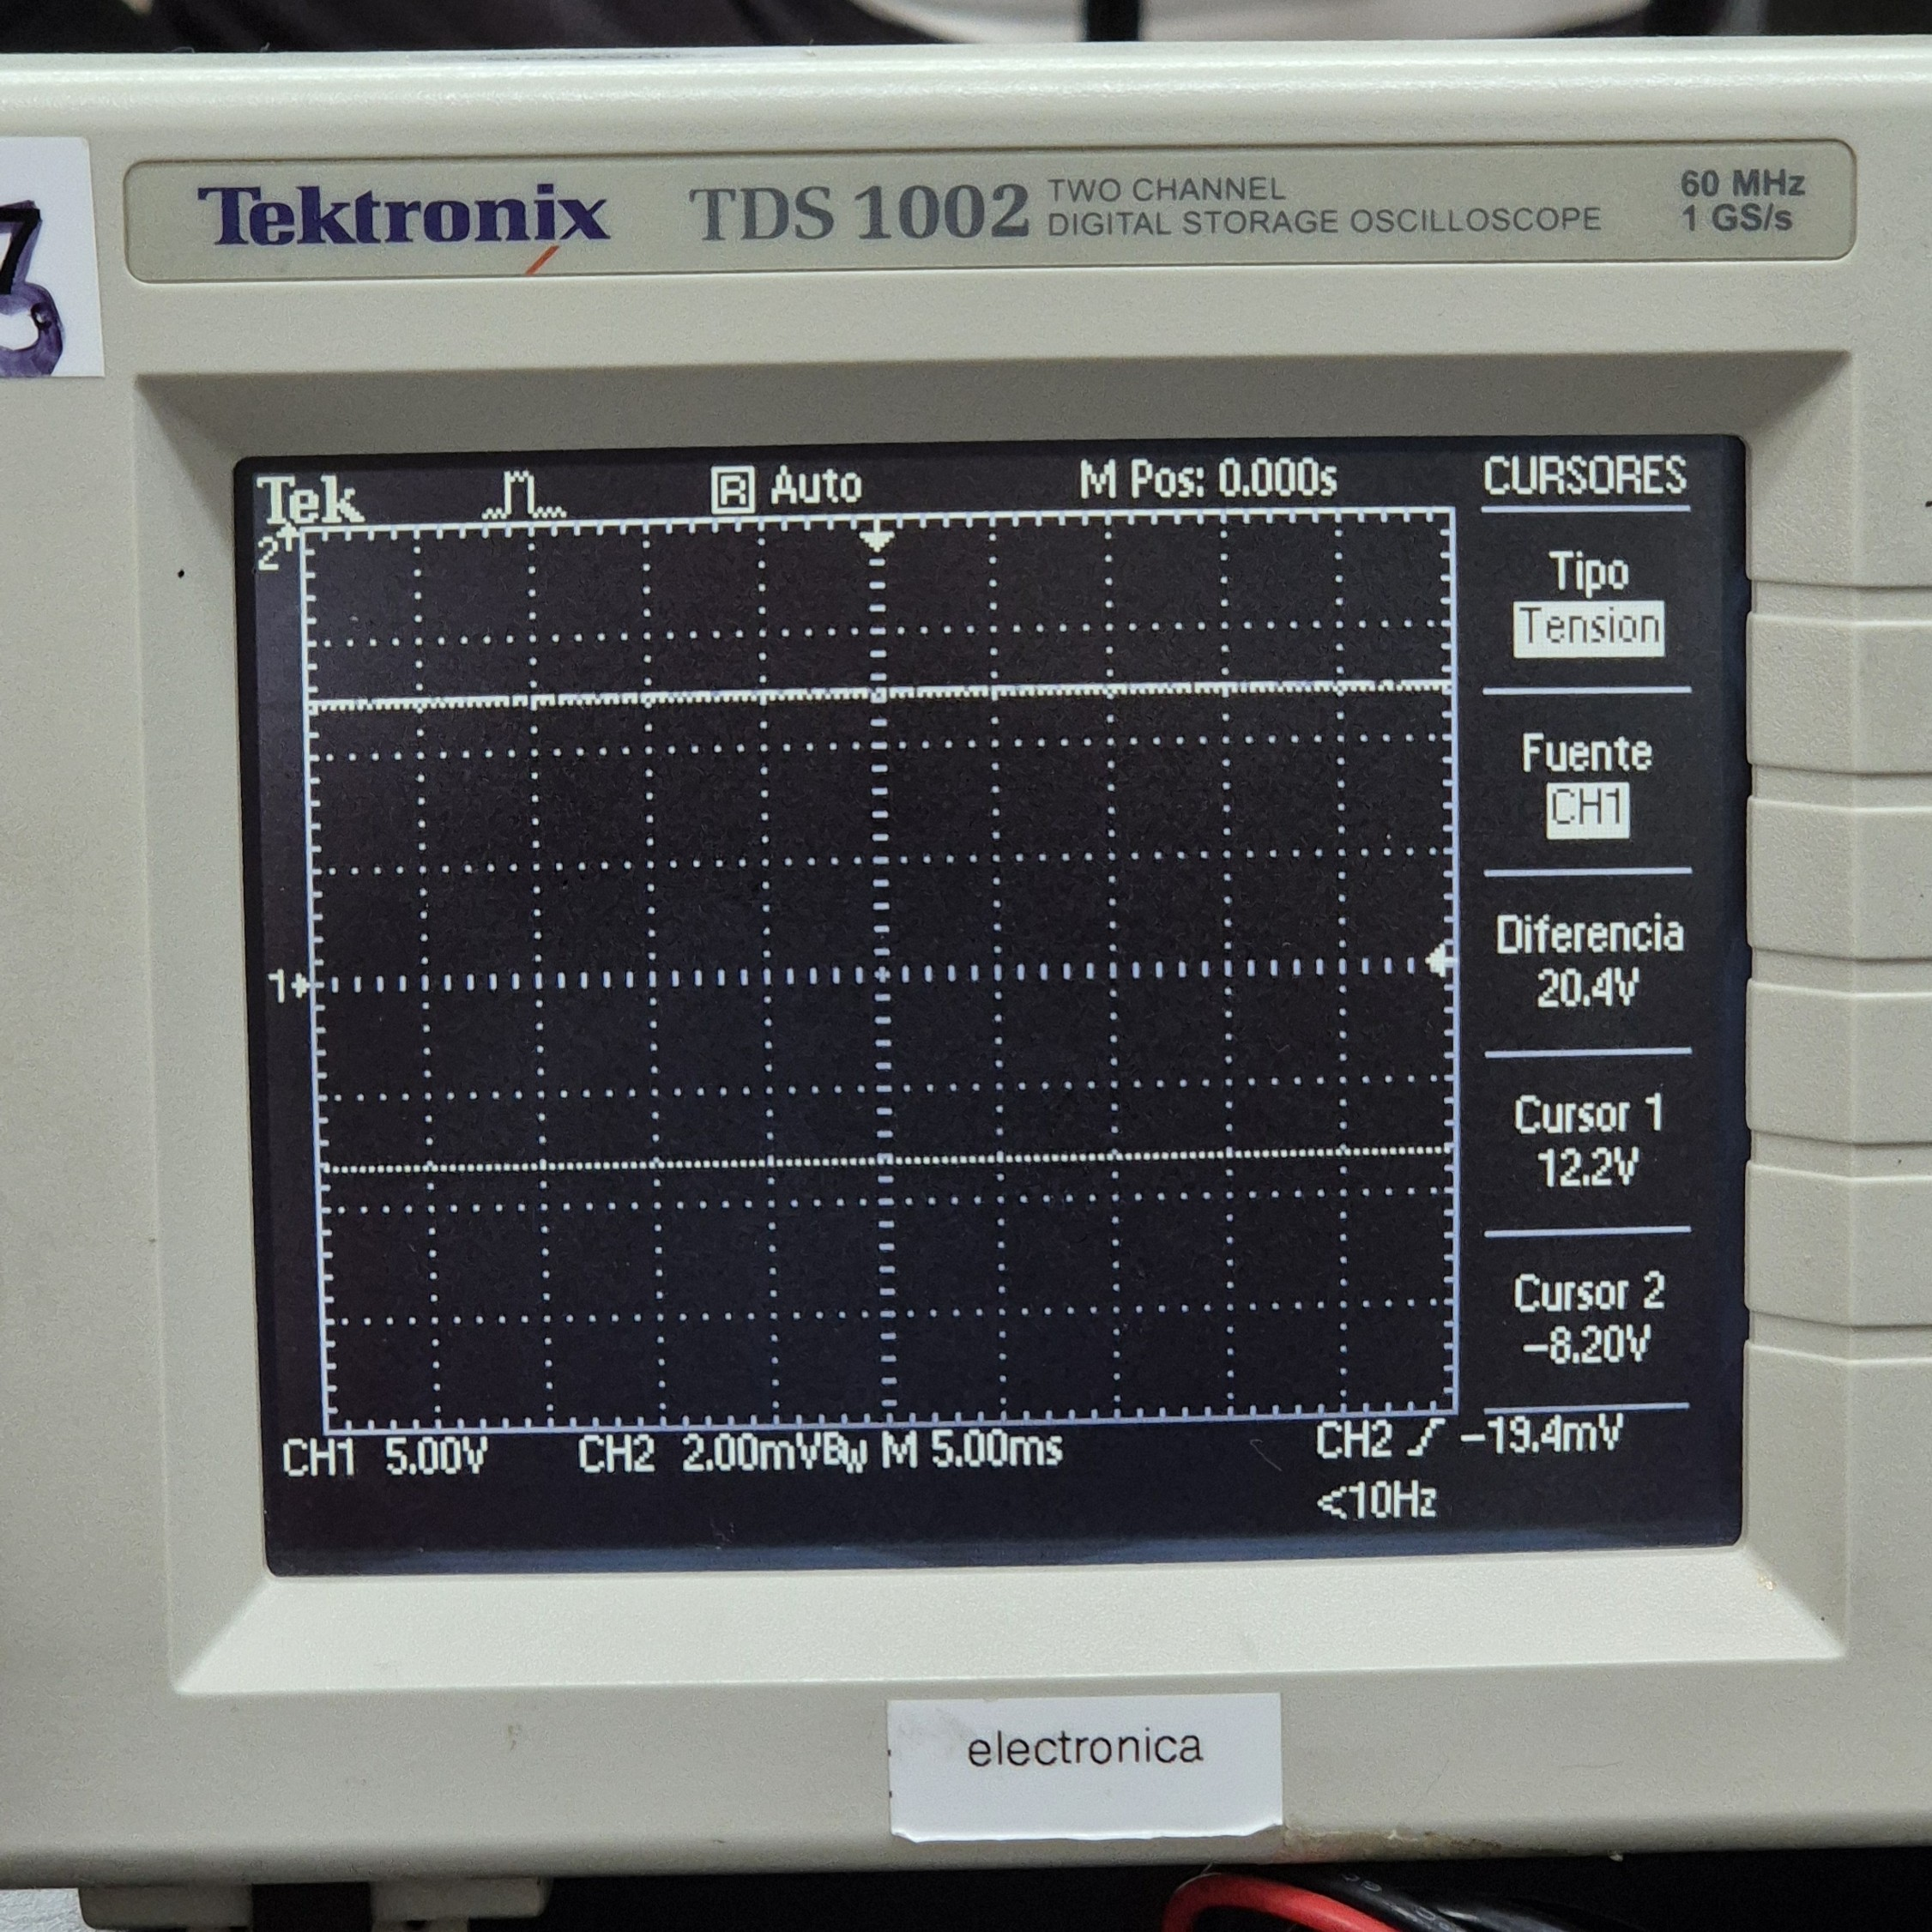
\includegraphics[width=0.42\textwidth]{imágenes/fuente DC/regulación.jpg}
				\caption{Señal obtenida luego de la Regulación con un regulador 7812.}
				\label{fig:regulador}
			\end{figure}

	\section{Fuente Simétrica}
		El siguiente objetivo fue realizar la Fuente Simétrica de la Figura \ref{fig:circuito_simétrica} (con valores distintos
		a la figura) que, dadas las etapas anteriormente realizadas para la fuente DC lineal, simplemente el circuito se
		``dividió en dos'', veámoslo.

		\begin{figure}[!ht]
			\centering
			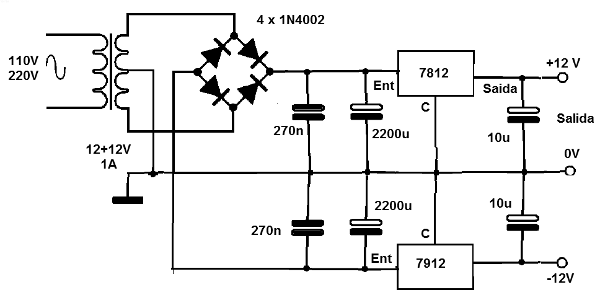
\includegraphics[width=0.48\textwidth]{imágenes/fuente simétrica/circuito.png}
			\caption{Circuito a montar (con valores distintos) para hacer una Fuente Simétrica a partir de una señal AC.}
			\label{fig:circuito_simétrica}
		\end{figure}

		La etapa de la Transformación se quedó casi identica, sin embargo, en esta ocasión las entradas de los extremos funcionaron
		como positivo y negativo, con ayuda del puente rectificador, y el tap central funcionó como la tierra.\\
		Asimismo, la Rectificación fue la misma, pero en este caso el puente rectificador separó el voltaje positivo del negativo
		del transformador, teniendo el tap central para la tierra.\\

		En el filtraje es más notoria la ``división'' del circuito en dos, pues en lugar de usar un capacitor y una resistencia
		se usaron dos de cada uno del mismo valor nominal, 1000 $\mu F$ y 3.9 $k\Omega$, acomodados de tal manera que un capacitor
		recibe el voltaje positivo y otro el negativo.\\
		Es importante destacar tener cuidado con la polaridad de los capacitores, pues el negativo de este se conecta a la parte
		más negativa del circuito, es decir, para el voltaje positivo la parte más negativa es la tierra y para el voltaje negativo
		la parte más negativa NO es la tierra, si no donde se encuentra el voltaje negativo.\\

		Finalmente, los reguladores, que para la parte positiva fue exactamente igual a la Fuente DC, sin embargo, para la parte
		negativa se usó otro regulador muy similar, el 7912, por lo cual se revisó el datasheet de este para corroborar valores de
		entrada y terminales.\\

		Finalmente se obtuvo como resultado lo mostrado en la Figura \ref{fig:simétrica}, que como podemos ver, se obtuvo un valor
		de voltaje simétrico, sin embargo, se obtuvo $\pm$ 9 $V$ lo cual es menor al esperado de acuerdo a los reguladores 7812 y 7912.

		\begin{figure}[!ht]
			\centering
			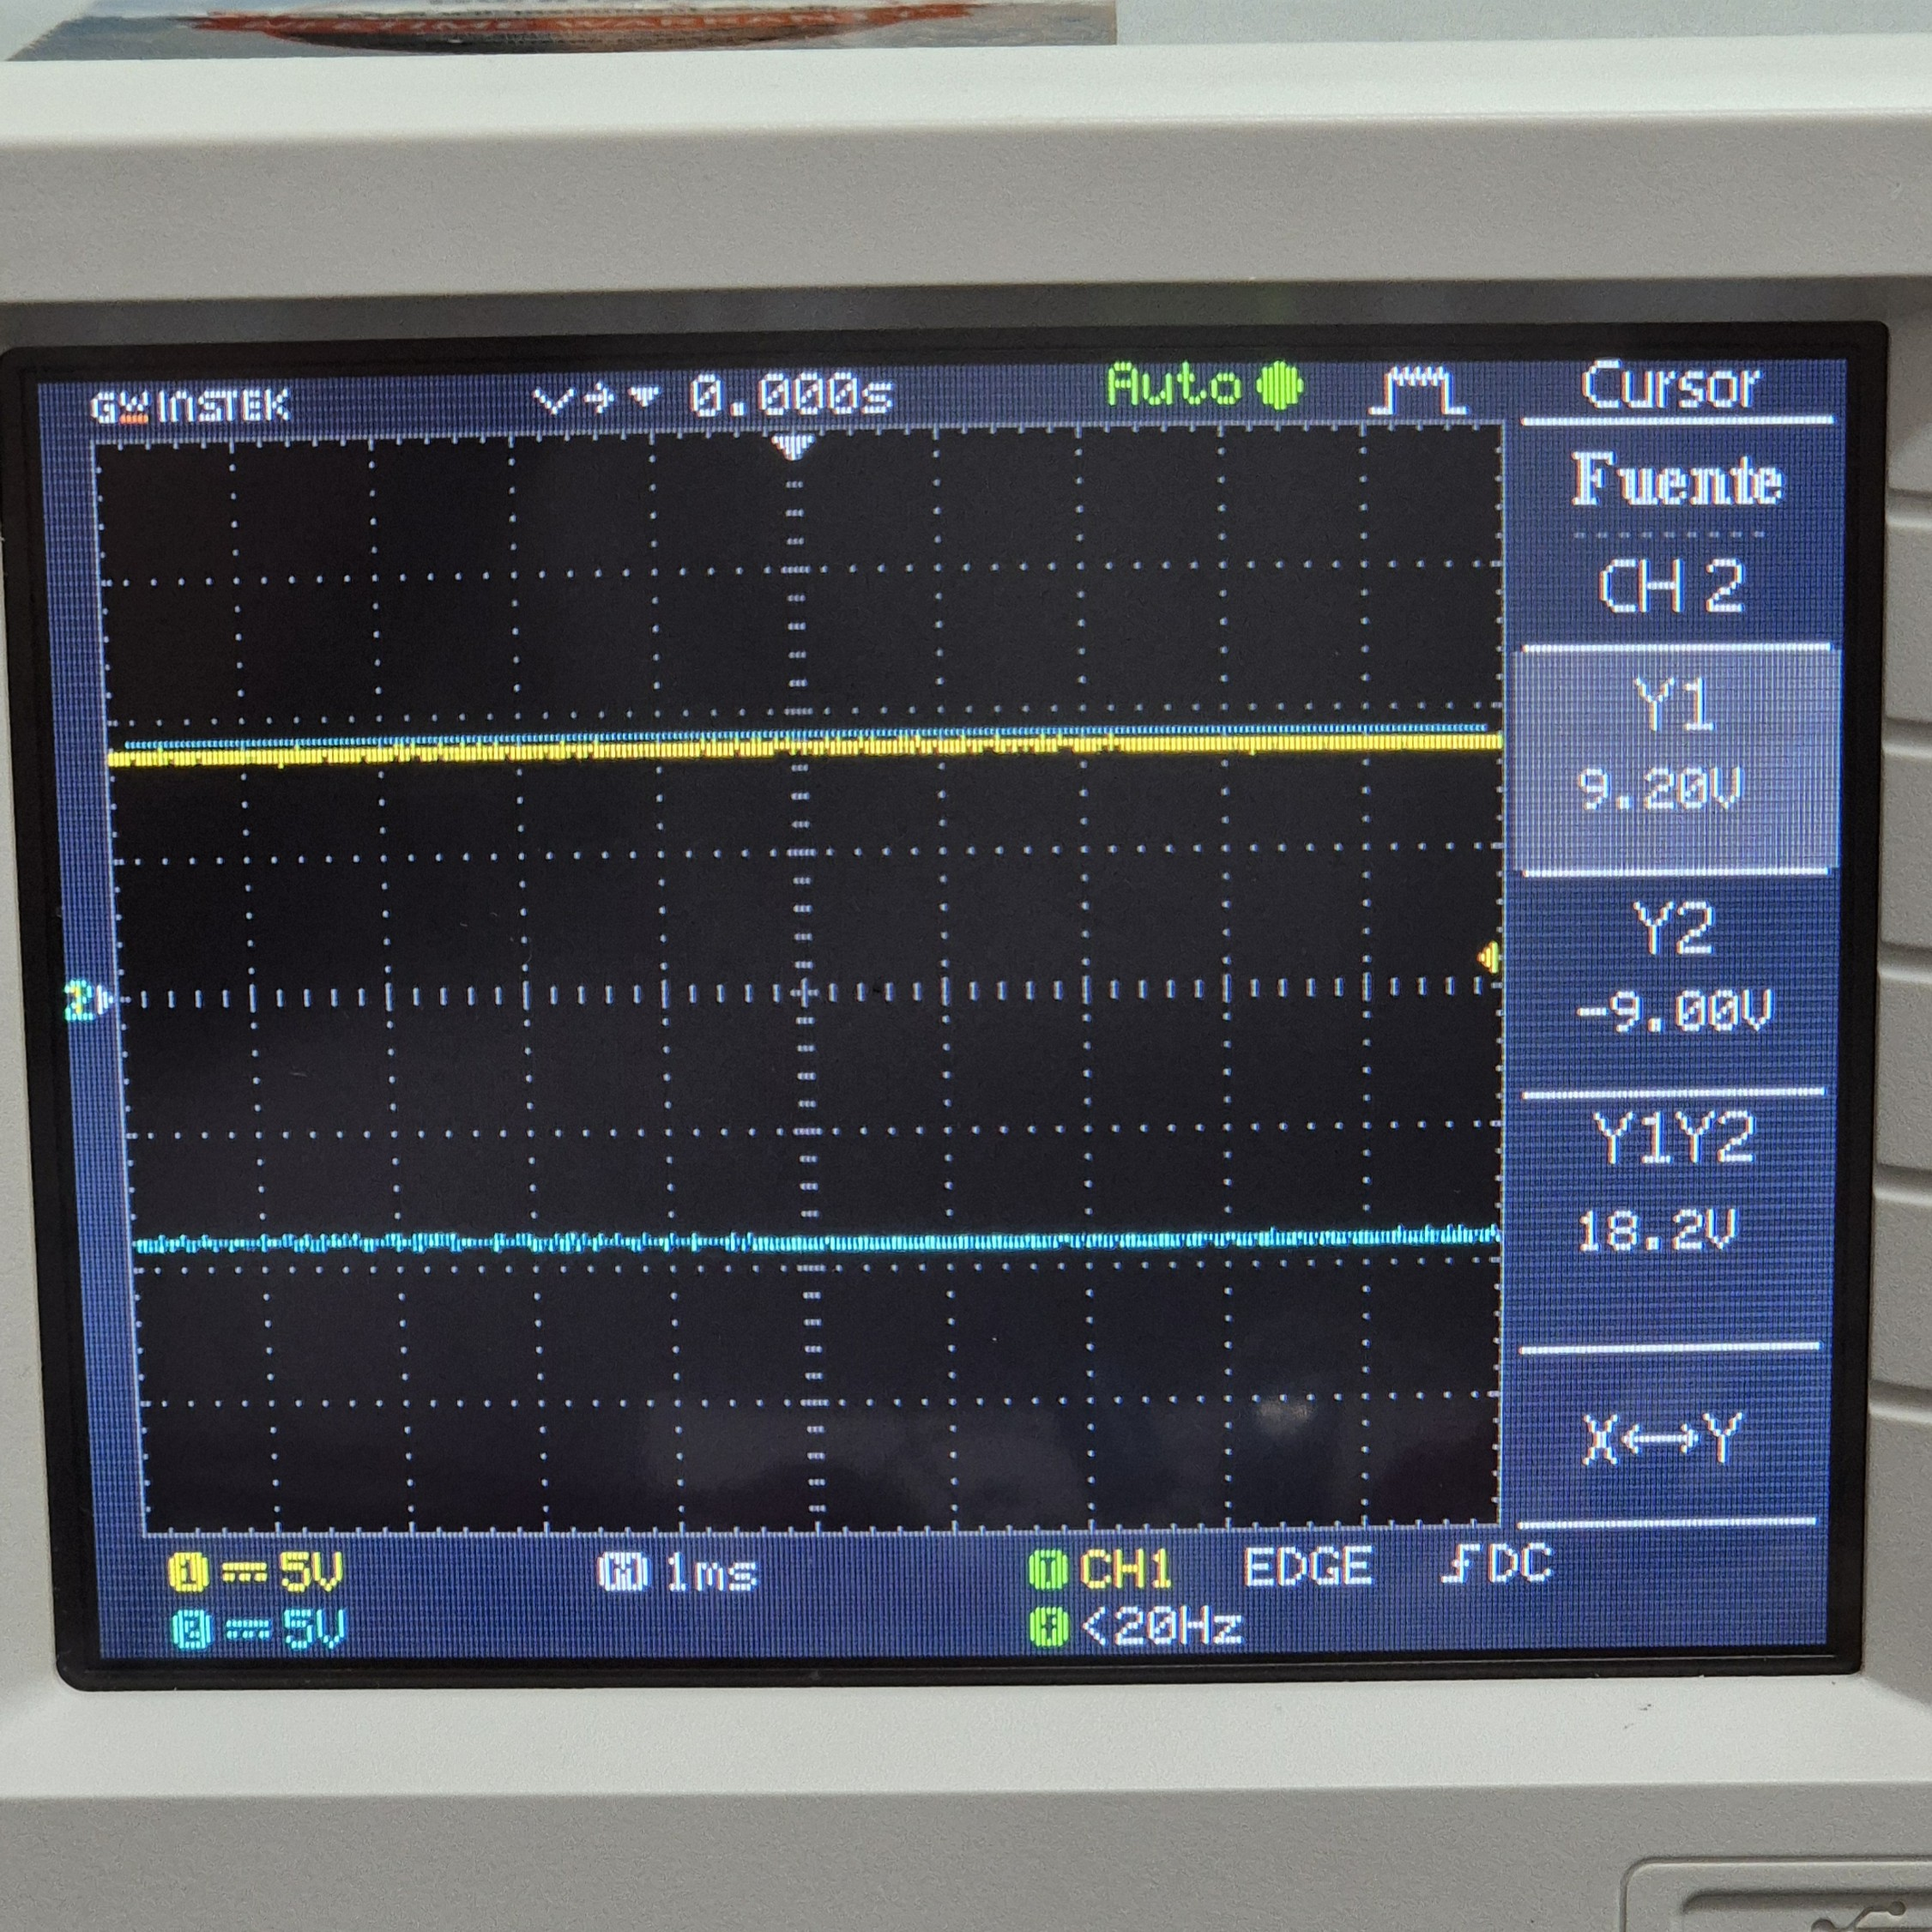
\includegraphics[width=0.48\textwidth]{imágenes/fuente simétrica/simétrica.jpg}
			\caption{Señal obtenida tras transformar la señal de la linea a una señal DC simétrica.}
			\label{fig:simétrica}
		\end{figure}

	% \printbibliography
	
\end{document}